%************************************************
\chapter{Curating a set of orthologous mammalian gene trees}
\label{ch_orthologs}
\acresetall
%************************************************
\section{The Mammalian Genome Project}

This chapter, Chapter \ref{ch_mammals1} and Chapter \ref{ch_mammals2}
describe different aspects of the research which the Goldman group and
I performed in collaboration with the \ac{mgp}. As a preface to these
chapters, here I introduce the \ac{mgp} and the main goals of the
analysis which was contributed to the consortium.

A major goal of mammalian comparative genomics has been to identify
and understand regions of the human genome that are evolving under
evolutionary constraint, as those regions are likely to be
functionally important \citep{Mouse2002Initial}. Protein-coding genes
clearly fall into this category, but additional non-coding functional
elements such as RNA genes, transcription factor binding sites, and
enhancer elements are known to also be functionally important and
subject to detectable purifying selection
\citep{Birney2007}. Comparisons of the first non-human mammalian
genomes to the human genome indicated that around 5\% of the human
genome has been evolving under purifying selection throughout the last
100 million years of evolution
\citep{Mouse2002Initial,Cooper2004,Rat2004Genome,LindbladToh2005Genome},
but the small number of genomes available at the time limited the
accuracy and resolution with which specific regions subject to
purifying constraint could be identified and classified
\citep{Ponting2011}.

The signal used to detect constrained regions is most commonly a
locally decreased rate of nucleotide substitutions
\citep{Cooper2004}. The strength of this signal increases along with
the expected number of substitutions per neutrally-evolving site
\citep{Siepel2005}, so the incorporation of additional genomes into
the analysis was expected to be an effective way to improve
power. Following this line of reasoning, the \ac{mgp} was proposed
with the primary goal of increasing the accuracy and confidence with
which evolutionarily constrained regions of the human genome could be
identified \citep{Margulies2005Initial,Margulies2007}.

The first phase of the \ac{mgp} took the form of a coordinated series
of genome sequencing projects initiated in 2005 and organised by the
Broad Institute of MIT and Harvard. In total, 20 new mammalian genomes
were sequenced, with species chosen in order to maximize the amount of
evolutionary divergence available for comparative analysis when
combined with the 9 mammalian genomes already available
\citep{Margulies2005Initial}. Most of the 20 additional species were
only sequenced to a target twofold coverage, meaning each genomic base
pair would be covered on average by two sequence reads and roughly
85\% of genomic sequence would be covered by at least one read. The
decision to sequence many genomes at low coverage was the result of a
deliberate compromise between the number of species sequenced and the
quality of each genome. The 2x level of coverage was estimated to
maximize the amount of additional branch length made available with a
reasonably high level of sequence quality given a limited budget
\citep{Margulies2007}.

As the project proceeded from its sequencing to analysis phase in late
2008, it became apparent that the additional branch length afforded by
the 29-species phylogeny would yield improved power for a number of
evolutionary analyses beyond the identification of constrained
non-coding regions. These included the evolutionary characterisation
of gene promoters, identification of exapted non-coding elements,
detection of evolutionary acceleration in non-coding regions, and
detection of purifying and positive selection in protein-coding
genes. Groups working on topics in these areas used the data generated
by the \ac{mgp} to conduct more focused analyses incorporating the
newly sequenced genomes. Given the prior involvement of the Goldman
group in analysing the comparative sequencing data from the
\ac{encode} project \citep{Margulies2007,Birney2007} and Tim
Massingham's work on the \ac{slr} method and software program
\citep{Massingham2005}, the group was recruited in late 2008 to
perform the protein-coding evolutionary analysis for the \ac{mgp} in
close collaboration with members of the Ensembl Compara team led by
Javier Herrero. The main goal was to use data from the newly sequenced
mammalian genomes to analyze selective pressures in proteins at the
level of individual codons. All of the work described in this and the
following two chapters was performed by me, though the work has
benefitted greatly from the advice and guidance of members of the
Goldman group (Nick Goldman, Tim Massingham and Ari L\"{o}ytynoja),
the EnsEMBL Compara team (Albert Vilella, Javier Herrero and Ewan
Birney) and various organisers and members of the \ac{mgp} (Manolis
Kellis, Kerstin Lindblad-Toh, Mike Lin and Katie Pollard).

\section{Introduction}

The main goal of the analysis presented in this and the following two
chapters was to characterize the amount and location of purifying and
positive selection within mammalian protein-coding genes. The primary
data were the genome sequences of the species being
compared. Originally, this consisted of the 29 Eutherian mammals
chosen for analysis by the \ac{mgp} consortium, but the analysis
described here used a larger group of 38 mammalian genomes included in
release 63 of the \ens database \citep{Flicek2011}.

In order to analyze proteins using phylogenetic codon models, a
significant amount of processing must be applied to the raw genomic
data. The annotation of protein-coding genes, identification of
orthologous sequences, and inference of phylogenetic trees and coding
alignments are all necessary steps in producing the inputs required
for analysis by methods such as \acs{paml} or \acs{slr}. The \ens gene
annotation and orthology pipelines already perform many of these steps
on a comprehensive set of mammalian and vertebrate genomes, so I used
the \ens databases as a source for gene annotations, gene trees, and
protein annotations where appropriate. In some cases, the \ens data
required modification or filtering: this chapter describes how
taxonomic constraints were used to extract a more useful set of
orthologous gene trees from the set of ``root'' phylogenetic trees
provided by \cmp, and Chapter \ref{ch_mammals1} describes how
sequences were extensively re-aligned and filtered before being
analyzed with \ac{slr}.

An important feature of the \ens gene annotation pipeline is that \lcv
genomes are processed using a modified version of the pipeline
designed to make the best possible use of the fragmented and gappy
assemblies resulting from \lcv shotgun genome sequences. This was a
significant factor behind my use of \ens as a primary source for gene
annotation and orthology information, as \ens is unique in
incorporating \lcv genomes into a full-fledged annotation
database. \citet{Hubbard2007} describe the modifications made to the
\ens pipeline to accommodate \lcv genomes, and I present the approach
and discuss some of its limitations in Section \ref{sec_ens_lcv}.

The main data used in the current chapter is the set of vertebrate
gene trees inferred by the \ens \cmp pipeline \citep{Vilella2009}. The
\cmp pipeline uses the set of annotated proteins within each
vertebrate genome to cluster homologs, align sequences and infer gene
trees with a Bayesian gene tree reconciliation method;
\citet{Vilella2009} describe and justify the approach and methods used
in the \cmp pipeline. This chapter begins with a description of the
methods used by the \cmp and other orthology pipelines, identifying
some aspects of the approach taken by \cmp which may have consequences
for my use of the gene trees to infer \sw selective pressures.

The gene trees inferred by the \cmp pipeline include a reconstruction
of the deep evolutionary history of genes, often containing paralogous
genes related by several ancient duplication events within one
phylogenetic tree. Many of the deep duplication events reflect the
\ac{2r} whole-genome duplication events that occurred in the
vertebrate ancestor, while more recent duplication events can be
viewed as part of an ongoing process of gene duplication and loss
within each genome. However, the inclusion of paralogous genes within
the current analysis was undesirable for two reasons. First, the goal
of this project within the scope of the \ac{mgp} was to use mammalian
evolutionary history to better understand the human genome, so gene
trees that represented largely orthologous evolutionary relationships
within mammals would provide the most useful context for understanding
our own genome. While ancient duplications are an interesting part of
the evolutionary history of genes, the evolution of duplicated genes
was beyond the scope of this analysis.

Secondly, a number of studies have suggested that duplicated genes may
evolve under different evolutionary constraints compared to singleton
genes in the genome. \citet{Dermitzakis2001a} showed that members of a
duplicate gene pair experienced different patterns of amino acid
changes linked to likely subfunctionalization \citep{Massingham2001},
and some studies have described increased rates of positive selection
within duplicate genes
\citep{Lynch2000,Zhang2002,He2005,Hahn2009a}. Although the extent to
which the evolution of paralogs differs from that of orthologs is a
matter of open debate \citep{Nembaware2002,Jordan2004,Studer2009}, the
potential for the adaptive evolution of duplicate genes to produce
misleading results in the current analysis made it important to avoid
including paralogous relationships within the gene trees to be
analyzed.

After introducing the methods behind the \cmp orthology pipeline, the
rest of this chapter presents an analysis of the set of gene trees
from version 63 of the \ens \cmp database and a description of the
method I used to extract a set of ``core'' orthologous gene trees for
further analysis. I show that the ``root'' \cmp trees encompass
various evolutionary distances (e.g., some trees included orthologs
linked by ancient duplication events, while others included only a
single set of orthologs), making it necessary to identify the set of
\subtr with appropriate orthologous characteristics. Although in
theory each \cmp tree contains a fully resolved history of gene
duplication and loss, in practice I found it unsatisfactory to use the
simplest imaginable approach---splitting each tree at all duplication
nodes---to extract a set of appropriate orthologs. Instead, I adopted
a method based on applying simple taxonomic constraints to identify
sub-trees with sufficient representation in the mammalian phylogeny to
warrant inclusion in the codon-based analyses described in the
following two chapters.

The major goals of the analysis presented here were to better
understand the distribution of orthologous genes within vertebrate
genomes, identify which taxonomic constraints would best identify
appropriate groups of mammalian orthologs within the \cmp gene trees,
and furthermore evaluate whether the genes annotated from \lcv
genomes, which are unique to the \cmp database, were of high enough
annotation quality and consistency to be included in the downstream
analysis. Throughout this chapter, attention is paid to those aspects
of the \cmp gene tree pipeline which may contribute to errors in the
downstream analysis.

\section{Methods for ortholog identification}

Central to most sequence analysis is the assumption that the sequences
being analyzed, or some parts therein, share a common evolutionary
origin. Thus, the first step in any such analysis is the collection of
homologous sequence data. Starting with a source sequence, putative
homologs are usually identified by searching a sequence database for
sequences with a minimum overall similarity according to some
evolutionary model. In some cases, such as when sequences are highly
divergent or subject to domain shuffling or horizontal gene transfer,
the idea of homology across an entire gene may be unsatisfactory and a
more localized concept of homology (based on shared domains or
functions) may be more appropriate
\citep{Koonin2001,Sjolander2011}. Within closely related groups of
organisms such as mammals, however, the process of gene duplication
and divergence dominates patterns of relatedness between protein
sequences \citep{Ohno1970}, making gene-wide sequence similarity a
useful method by which to identify homologous sequences in the
organisms of interest.

Heuristic algorithms have been developed for performing quick and
sensitive sequence homology searches within databases of protein and
nucleic acid sequences \citep{Altschul1997,Eddy2009}. The power of
these methods is high enough that homology within vertebrates, even
for fast-evolving genes, can be readily detected. However, the
prevalence of historical and ongoing gene duplication and loss in
vertebrates complicates the problem, as orthologous genes (e.g.,
homologs between species sharing a common ancestral population and
related through a speciation event) and paralogous genes (e.g.,
homologs sharing a common ancestral genomic sequence and related
through a duplication event) are important yet difficult to
distinguish from one another \citep{Jun2009}. In other words, sets of
genes that may be confidently identified as sharing homology may still
contain paralogy and orthology relationships that are more difficult
to resolve. Since the evolutionary trajectories of paralogous versus
orthologous genes are expected to be quite distinct \citep{Lynch2000},
the correct identification of orthologous versus paralogous
relationships in vertebrates is critical for any detailed molecular
evolutionary analysis.

Many methods for distinguishing orthologous from paralogous
relationships within vertebrate genomes have been developed over the
past decade \citep{Yuan1998,Remm2001}, but the amount of overlap
between vertebrate orthologous groups identified by different methods
has historically been disappointingly small \citep{Chen2007,Jun2009},
suggesting that the problem of orthology inference is far from
resolved. Still, one might expect the accuracy and power of orthology
inference methods to improve with time, given the steady increase in
available computing power and the sequencing of many complete
vertebrate genomes over the past decade. Complete genomes are
important in that the availability of a complete set of genes allows
for duplication and loss events to be more confidently inferred. The
growing number of available sequenced genomes, greater available
computational power, and improved understanding of patterns of gene
duplication and loss have led to the growing popularity of
phylogeny-based approaches, which were once considered computationally
impractical and too difficult to automate \citep{Remm2001}. In
general, the phylogenetic approach involves estimating a phylogenetic
tree from an entire cluster of homologous genes and inferring
duplication events based on the discordance between the gene tree and
the species tree. This approach is most powerful when the species tree
can be confidently estimated, though some methods allow for species
tree uncertainty \citep{Vilella2009} and there is not too much
uncertainty in the relationships between most mammals. Several
variants of this approach have been developed and applied to gene tree
reconstruction in insects, fungi and vertebrates
\citep{Muller2010a,Cepas2007,Datta2009,Vilella2009,Ruan2008,Hahn2007a},
and validation against manually-curated gene trees has shown these
phylogeny-based methods to be more sensitive and accurate than
pairwise or graph-based methods \citep{Datta2009}.

The \cmp pipeline uses TreeBeST, a phylogeny-based method which uses a
known species tree to guide the resolution of orthologs and paralogs
within a gene tree in a Bayesian framework, to infer its gene trees,
so I will refer mainly to this method throughout the rest of this
chapter. TreeBeST is one of the more popular phylogeny-based methods,
having also been used to infer vertebrate and eukaryotic gene trees
for the OPTIC and TreeFam databases
\citep{Heger2008,Ruan2008,Vilella2009}.

\section{Low-coverage genomes in the Ensembl database}
\label{sec_ens_lcv}

A major feature that distinguishes \cmp from the Treefam and Optic
databases is the inclusion in \cmp of several mammalian genomes which
were sequenced to low coverage by the \ac{mgp}. The inclusion of these
additional genomes was a major reason why I performed the analysis
described in the following chapters using Ensembl as a source of gene
trees and alignments, representing a major advantage over otherwise
similar orthology databases due to the greater species sampling
density. 
%Here I provide some more detail on the way \lcv genomes are
%handled within the Ensembl annotation pipeline, as certain features of
%the \lcv genomes cause characteristic anomalies in the orthology
%analyses.

The prevalence of missing sequence data and fragmented contigs in \lcv
genomes presents a unique set of problems for the generation of
transcript annotations in \ens, so the procedure used by \cmp to
annotate genomes assembled from \lcv data is distinct from the usual
gene-building pipeline \citep{Hubbard2007}. Although the ``normal''
annotation pipeline varies somewhat between different high-coverage
genomes, the general approach taken is to align experimentally
observed transcripts and protein sequences from a variety of sources
against the new genome in order to infer gene and transcript
structures. The main difference for the \lcv genomes is that a
whole-genome alignment is produced between the human genome and each
\lcv target genome, and gene models are projected from human to the
target genome. Small frame-disrupting insertions or deletions within
orthologous exons are then corrected, and missing or incomplete exons
are padded with Ns in order to produce a transcript with a length
equal to that of the human reference transcript. The inclusion of
these error-correcting features allows for a set of intact, if not
complete, coding transcripts to be generated for \lcv genomes,
leveraging the high level of sequence similarity between human and
other \euth mammals to project genes and transcripts from the
high-quality human genome to the unannotated, highly fragmented \lcv
genome assemblies. 

Still, in many cases the \ens pipeline cannot map complete genes or
transcripts from human to the target genome, causing difficulty in
identifying duplications \citep{Hubbard2007}. On one hand, the lack of
completely assembled chromosomes means that segmental duplications in
\lcv genomes are often unresolved or unidentifiable, making it
difficult or impossible to confidently identify recently duplicated
genes. On the other hand, the shorter length of assembled fragments
causes genes to occasionally be split between two sequence fragments;
the \ens pipeline currently annotates such genes as two separate
shortened gene fragments, resulting in an excess of shortened apparent
paralogs in the resulting gene trees.
% (see Section
%\ref{sec_removing_paralogs} for more detail on this artifact).

The \cmp gene family pipeline uses the set of annotated transcripts
from each species as its input \citep{Vilella2009}, so the quality of
gene annotation from each source genome has a direct impact on the
overall quality and accuracy of the resulting gene trees which formed
the source data for my analysis. Although the reliance on genome-wide
alignments to, and gene annotations from, a reference genome could be
criticized for potentially causing a bias towards the genomic
properties of the reference, this approach is a reasonable workaround
in the absence of higher-coverage sequence data or a painstakingly
curated assembly. Furthermore, the gene model error-correcting
features of the Ensembl pipeline are especially beneficial, making
more complicated methods for correcting sequencing errors from \lcv
genomes such as those described by \citep{Hubisz2011} seem less
necessary.

\section{The Ensembl Compara gene tree pipeline}
\label{sec_compara_pipeline}

All genomic data and gene trees used for this analysis were sourced
from version 63 of the Ensembl Compara database
\citep{Vilella2009,Flicek2011}. Although a complete description of the
design, implementation, and validation of the pipeline behind the
Ensembl database is beyond the scope of this chapter, I will briefly
outline the major aspects of the approach used by the Compara gene
tree inference pipeline, focusing on a few key details which are
relevant to the current analysis.

The Compara pipeline begins with a set of protein-coding transcripts
collected from each individual species' annotation database. This step
is not straightforward, however, as the prevalence of alternative
splicing in \euth mammals makes it common for a single gene to harbor
many different transcript structures.

%As an aside, it is worth mentioning that in terms of mammalian biology
%and evolution, alternative splicing is a very interesting
%phenomenon. Tightly linked to the evolutionary innovation of
%regulatory control and tissue-specific gene expression, the existence
%of multiple transcripts per gene is one of the likely substrates of
%biological and developmental complexity within vertebrates and mammals
%as compared to single-celled eukaryotes, which show less developmental
%complexity but largely similar numbers of genes
%\citep{Csuros2011}. Further evidence of the unique evolutionary
%characteristics of alternatively-spliced exons comes from molecular
%evolutionary studies which have shown such exons to show, on average,
%higher levels of evolutionary constraint, possibly owing to the
%importance of exonic splice enhancers in modulating the inclusion or
%exclusion of their associated exons \citep{Parmley2006}.

%In terms of organizing biological data, however, 

The pervasiveness of alternative splicing is somewhat burdensome for a
comparative analysis of genes. Roughly 34\% of human genes contain at
least two, and up to several dozen, transcripts per gene
\citep{Mironov1999}, showing tissue-specific and species-specific
expression patterns, different levels of overall transcription, and
sometimes comprising mutually exclusive exons. Within the context of
the \cmp database, the first problem in maintaining consistency across
many source genome sequences is the fact that primary data on
alternative transcript structures (e.g., data from expressed sequence
tags, RNA-seq, or proteomics experiments) are largely absent from most
organisms with sequenced genomes. Furthermore, the task of
incorporating multiple transcripts per gene into an evolutionary
framework is non-trivial, and leaves many unresolved questions open to
debate: should all transcripts be treated as independent evolutionary
entities, or should some form of meta-transcript be produced,
comprising all possible transcripts for a given gene? Should
expression levels and tissue-specificity be taken into account (as
both factors have been correlated with evolutionary rate,
e.g. \citep{Koonin2006a,Zhu2008})? And what is the expected
evolutionary impact of the loss, gain, or modulation of the prevalence
or tissue-specificity of a given exon or transcript in one lineage?
Even a fairly shallow consideration of the topic quickly reveals
layers of complexity that would quickly hinder many large-scale
evolutionary analyses, such as the definition of orthologous groups,
whose main goals are to understand the evolutionary relationships of
gene families within some set of species' genomes.

Returning to the description of the \cmp pipeline, I note that it
currently only includes one ``canonical'' transcript per gene in the
clustering tree-building process. This reflects a conscious decision
to sacrifice some biological fidelity for reduced design complexity
and computational load, as the inclusion of multiple transcripts would
inevitably require some amount of additional processing and/or
calculation. Unfortunately, this only somewhat alleviates the problem,
shifting the burden from ``how to deal with multiple transcripts in a
comparative setting'' to ``how to choose the best representative
transcript for each gene.'' In the case of a gene with many
transcripts of varying sizes containing many non-overlapping exons,
the consequences of choosing a non-optimal transcript are clear: too
short of a transcript could exclude important sequence information
from the dataset, while transcripts with spurious exons (resulting
from misannotation or erroneous experimental evidence for a
transcript) could introduce potentially large amounts of
non-orthologous, nonfunctional, or nonconserved sequence into the
evolutionary analysis.

Fortunately, the consensus coding sequence (CCDS) project was
initiated in 2005 to ``identify a core set of human and mouse protein
coding regions that are consistently annotated and of high quality''
\citep{Pruitt2009}. Although the transcripts that satisfy these two
criteria will not necessarily be the same as those which meet the
desired definition of ``the best representative transcript for use in
an evolutionary study,'' the confidence that one can have in the
quality and consistency of CCDS transcripts helps to reduce the
prevalence of potentially damaging errors in the Compara pipeline.
Thus, in the current release (version 63), the ``representative''
transcript used for the Compara pipeline is chosen on the basis of (a)
existence within the CCDS set of transcripts and (b) the total length
of the transcript's coding sequence. The combination of these two
factors can be expected to identify a reasonably representative
transcript, at least for the human and mouse genomes. The situation
will be similar for genomes whose Ensembl annotation is derived
largely from synteny and orthology to human and mouse annotated genes,
but two classes of genomes---those resulting from low-coverage
sequencing and those from more distant species whose annotations are
derived from largely independent data sources---will still suffer from
some amount error due to transcript choice. In comparison, the OPTIC
database, which contains orthologous groups identified within a wide
range of animal and fungal clades, uses the transcript with the
maximum length as the canonical transcript \citep{Heger2008}.

Once the set of canonical transcripts is chosen, the \cmp pipeline
performs an all-against-all protein BLAST search is performed using
the Washington University variant of BLAST \citep{Chao1992} and genes
are clustered into homologous groups using \hclust \citep{Ruan2008},
an implementation of a hierarchical clustering algorithm for sparse
graphs which is distributed with the widely-used TreeBeST
package. Sequences are aligned using MCoffee, a meta-aligner algorithm
which combines the results from different aligners into one alignment
using a maximum-consistency criterion \citep{Wallace2006}. The
aligners used for the M-Coffee alignment include MAFFT
\citep{Katoh2005}, MUSCLE \citep{Edgar2004}, KAlign
\citep{Lassmann2009}, and T-Coffee \citep{Notredame2000}. Finally, the
aligned sequences are input to TreeBeST, which infers a gene tree
(including gene duplication and loss events) given a set of aligned
sequences and a known species tree \citep{Ruan2008}. The type of the
homology relationship between each pair of genes (e.g., one-to-one
ortholog, one-to-many ortholog, within-species paralog) is determined
using a simple set of rules based on the structure of the inferred
gene tree and the annotation of ancestral nodes where a duplication
event has likely occurred.

%The Compara pipeline has been a part of the Ensembl ecosystem since
%its first introduction to Ensembl in release 42
%\citep{Birney2006}. Remarkably, aside from slight tweaks to the
%protein clustering method and some changes in the exact aligners used,
%the pipeline has changed little from its original published form
%\citep{Vilella2009}. In part, this lack of change reflects the ease
%with which sets of vertebrate orthologs can be identified using the
%existing methodology, lying in contrast to the equivalent task in sets
%of insect or fungal genomes where divergence levels between extant
%species with sequenced genomes are much larger \citep{Siepel2005} and
%the shape of the underlying species tree may be uncertain and/or
%unknown \citep{MacKenzie2008a}, making the development of specialized
%methods or extensive manual annotation necessary
%\citep{Kellis2004,Rasmussen2007}. This is equivalent to saying that
%Ensembl's pipeline, while not perfect in its orthology predictions or
%tree inferences (as indicated in a series of back-and-forth papers
%between \citet{Milinkovitch2010} and \citet{Vilella2011}), has proved
%sufficiently accurate enough that an extensive reworking of the system
%has not yet been deemed necessary. However, it is worth noting that
%the recent development of a new Bayesian method for gene tree
%reconciliation, based on a generative model of gene family evolution
%as a birth-death process and incorporating species-specific and
%gene-specific rate variation, showed good performance in resolving
%fungal and invertebrate gene trees, and could easily be adapted to the
%vertebrate genomes in the Compara database
%\citep{Rasmussen2011}. Additional validation of the overall approach
%taken by Compara comes in the form of Treefam and OPTIC
%\citep{Ruan2008,Heger2008}, databases of animal and fungal gene trees
%which applied a similar set of tools to infer gene trees from a more
%diverse set of genomes \citep{Vilella2009}.

\section[Quantifying paralogous relationships within Ensembl gene trees]{Quantifying paralogous relationships within \\ Ensembl gene trees}
\label{section_quantifying_paralogous}

As stated in the introduction, the main goal of this chapter was to
identify and extract a set of gene trees or gene \subtr{}s from the
\cmp database comprising largely of orthologous relationships within
mammals, avoiding as much as possible the inclusion of paralogous
relationships. I will refer to trees with these characteristics as
\acp{lot}.

It was necessary to use some sort of criterion to extract \acp{lot}
from the set of \cmp gene trees, because many of the \cmp trees
contained multiple sets of complete \mammln orthologous trees linked
by ancient gene duplication events. In other words, the Compara gene
trees could be characterized as being over-clustered with respect to
the core set of \mammln orthologous trees. This over-clustering was
not necessarily inaccurate with respect to the evolutionary history of
vertebrate genes, but it was not a desirable feature for my intended
use of the data. This section is concerned with quantifying the amount
of this over-clustering within the Compara database.

I first collected the set of 18,607 \cmp gene trees and analyzed their
overall size and the number of human genes contained within each
tree. The results of this analysis are presented in Table
\ref{table_ensembl_roots} and Figure \ref{fig_ensembl_roots_hist}; a
complete description of these data will follow in Section
\ref{section_root_compara_trees}, but the aspects relevant to
characterizing the amount of paralogy contained within these trees
will be discussed here.

The first row of Table \ref{table_ensembl_roots} shows various summary
statistics from the full set of \cmp gene trees, with the columns
under the ``Human Content'' heading showing the fraction of all gene
trees containing zero, one, or two or more human genes. Evidence for
the existence of large numbers of paralogs within \cmp trees came from
the observation that 20\% of \cmp trees contained 2 or more human
genes. If each Compara tree contained only one set of \mammln
orthologs, then the 20\% of trees with multiple human gene copies
could only be explained by an unrealistically high rate of gene
duplication in the lineage leading towards human. Instead, a more
parsimonious explanation was that many of the Ensembl trees contained
not one group of \mammln \acp{lot}, but two or more sets of \mammln
\acp{lot} joined by one or more ancient duplication events. This
explanation was further supported by Figure \ref{fig_ensembl_roots_hist},
which shows a histogram of total gene counts in the Ensembl root
trees. A large number of trees contained more than 48 sequences (the
number of vertebrate genomes in \ens), with clear peaks in the
histogram of trees with 2, 3, and 4 times the number of vertebrate
genomes in \ens. These patterns were highly consistent with a large
number of \cmp gene trees containing multiple \mammln \acp{lot}.

\begin{table}
\scriptsize \centering
\begin{tabular}{lrb{2cm}rrrrrrrr}
\toprule
 & Tree &  \multicolumn{3}{c}{Sequence Counts} & \multicolumn{3}{c}{Human Content} & Human & Med. & Med. \\ \cmidrule(r){3-5} \cmidrule(r){6-8}
Tree Set & Count  & \tiny{Med (Min / Max)} & Total & N50 & 0 & 1 & 2+ & Total & MPL & Species \\ 
  \midrule
\input{Tables/ortholog_roots_summary.txt}
   \bottomrule
\end{tabular}
\caption{Summary of the set of Ensembl Compara root trees. The ``Human
  Content'' columns represent the fraction of trees which contain the
  indicated number of human genes, and ``Human Total'' is the total
  number of human genes contained within the tree set. ``Med. Species''
  is the median species count across all trees. Med.---median;
  MPL---mean path length.}
\label{table_ensembl_roots}
\end{table}


The prevalence of over-clustered \euth orthologs in the Compara
database could be explained by a combination of the \hclust algorithm
used for the hierarchical clustering step, which uses only protein
distances as its source of clustering information, and the wide range
of protein evolutionary rates in the vertebrate genome. The Compara
pipeline uses an all-by-all protein BLAST search and the \hclust
algorithm to produce sets of clustered sequences. To identify
clusters, the \hclust algorithm uses E-scores resulting from each
pairwise BLAST result, where the E-score represents the expected
number of unrelated sequences which would produce equal or higher
similarity scores in the given database. Clusters are chosen to
produce groups of sequences with minimal average within-group
E-values. No additional biological information, such as the source
species of each sequence or the overall \acl{tc} of each cluster, is
used in identifying clusters, and no attempt is made to fit clusters
to an expected model of orthologous gene evolution. On the one hand,
the lack of additional information and assumptions allows the
algorithm to remain simple and the clustering behavior to remain
consistent across different groups of genomes; on the other hand, a
number of technical (in the sense of non-biologically meaningful)
parameters and thresholds must be tuned in order to result in the
desired cluster sizes and contents. Importantly, even after these
parameters were tuned to successfully cluster a majority of vertebrate
orthologs, the reliance on protein distances alone means that
fast-evolving proteins will be more likely to be under-clustered and
slow-evolving proteins will be more likely to be over-clustered. The
rate of protein evolution varies widely within a genome, as evidenced
by a study of amino-acid substitution rates of roughly 6,000
eukaryotic orthologous genes \citep{Koonin2004}, which found that the
middle 90\% of genes show a nearly fourfold variation in evolutionary
rate. Given this wide range of protein evolutionary rates, the excess
of over-clustered orthologs in the Compara database is understandable
and even somewhat expected.

\begin{figure}
\centering
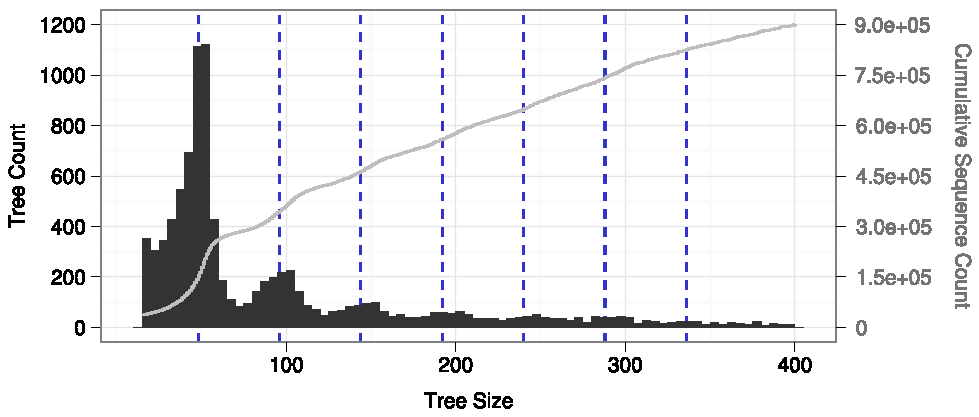
\includegraphics[scale=0.9]{Figs/hist_ens_roots.pdf}
\caption{Tree sizes for the set of ``root'' Compara trees. Black bars
  show a histogram of tree sizes in bins of width 5, and a gray line
  shows the cumulative number of sequences contained within trees of
  that size or smaller. For clarity, 9,378 trees with 15 or fewer
  sequences are not shown (but they have been included in the
  calculation of the cumulative sequence count). Dashed blue lines are
  drawn at integral multiples of 48, the number of vertebrate species
  within Ensembl.}
\label{fig_ensembl_roots_hist}
\end{figure}


Before continuing with a description of a method to identify \acp{lot}
within \cmp gene trees, I should note that my use of the phrase
``over-clustered'' refers only to over-clustering with respect to the
current goal of analyzing independent sets of orthologous genes within
\mamml{}s. Certainly these large ``over-clustered'' trees, which
represent a more distant evolutionary history than a single \mammln
orthologous group, are just as accurate with respect to the true
evolutionary history of the genes as more narrow groupings would
be. Furthermore, the inclusion of a deeper evolutionary context may
sometimes be more useful to users of the Compara database, for whom an
understanding of the overall evolutionary history of a gene may be the
topic of primary interest.

\begin{figure}
\centering
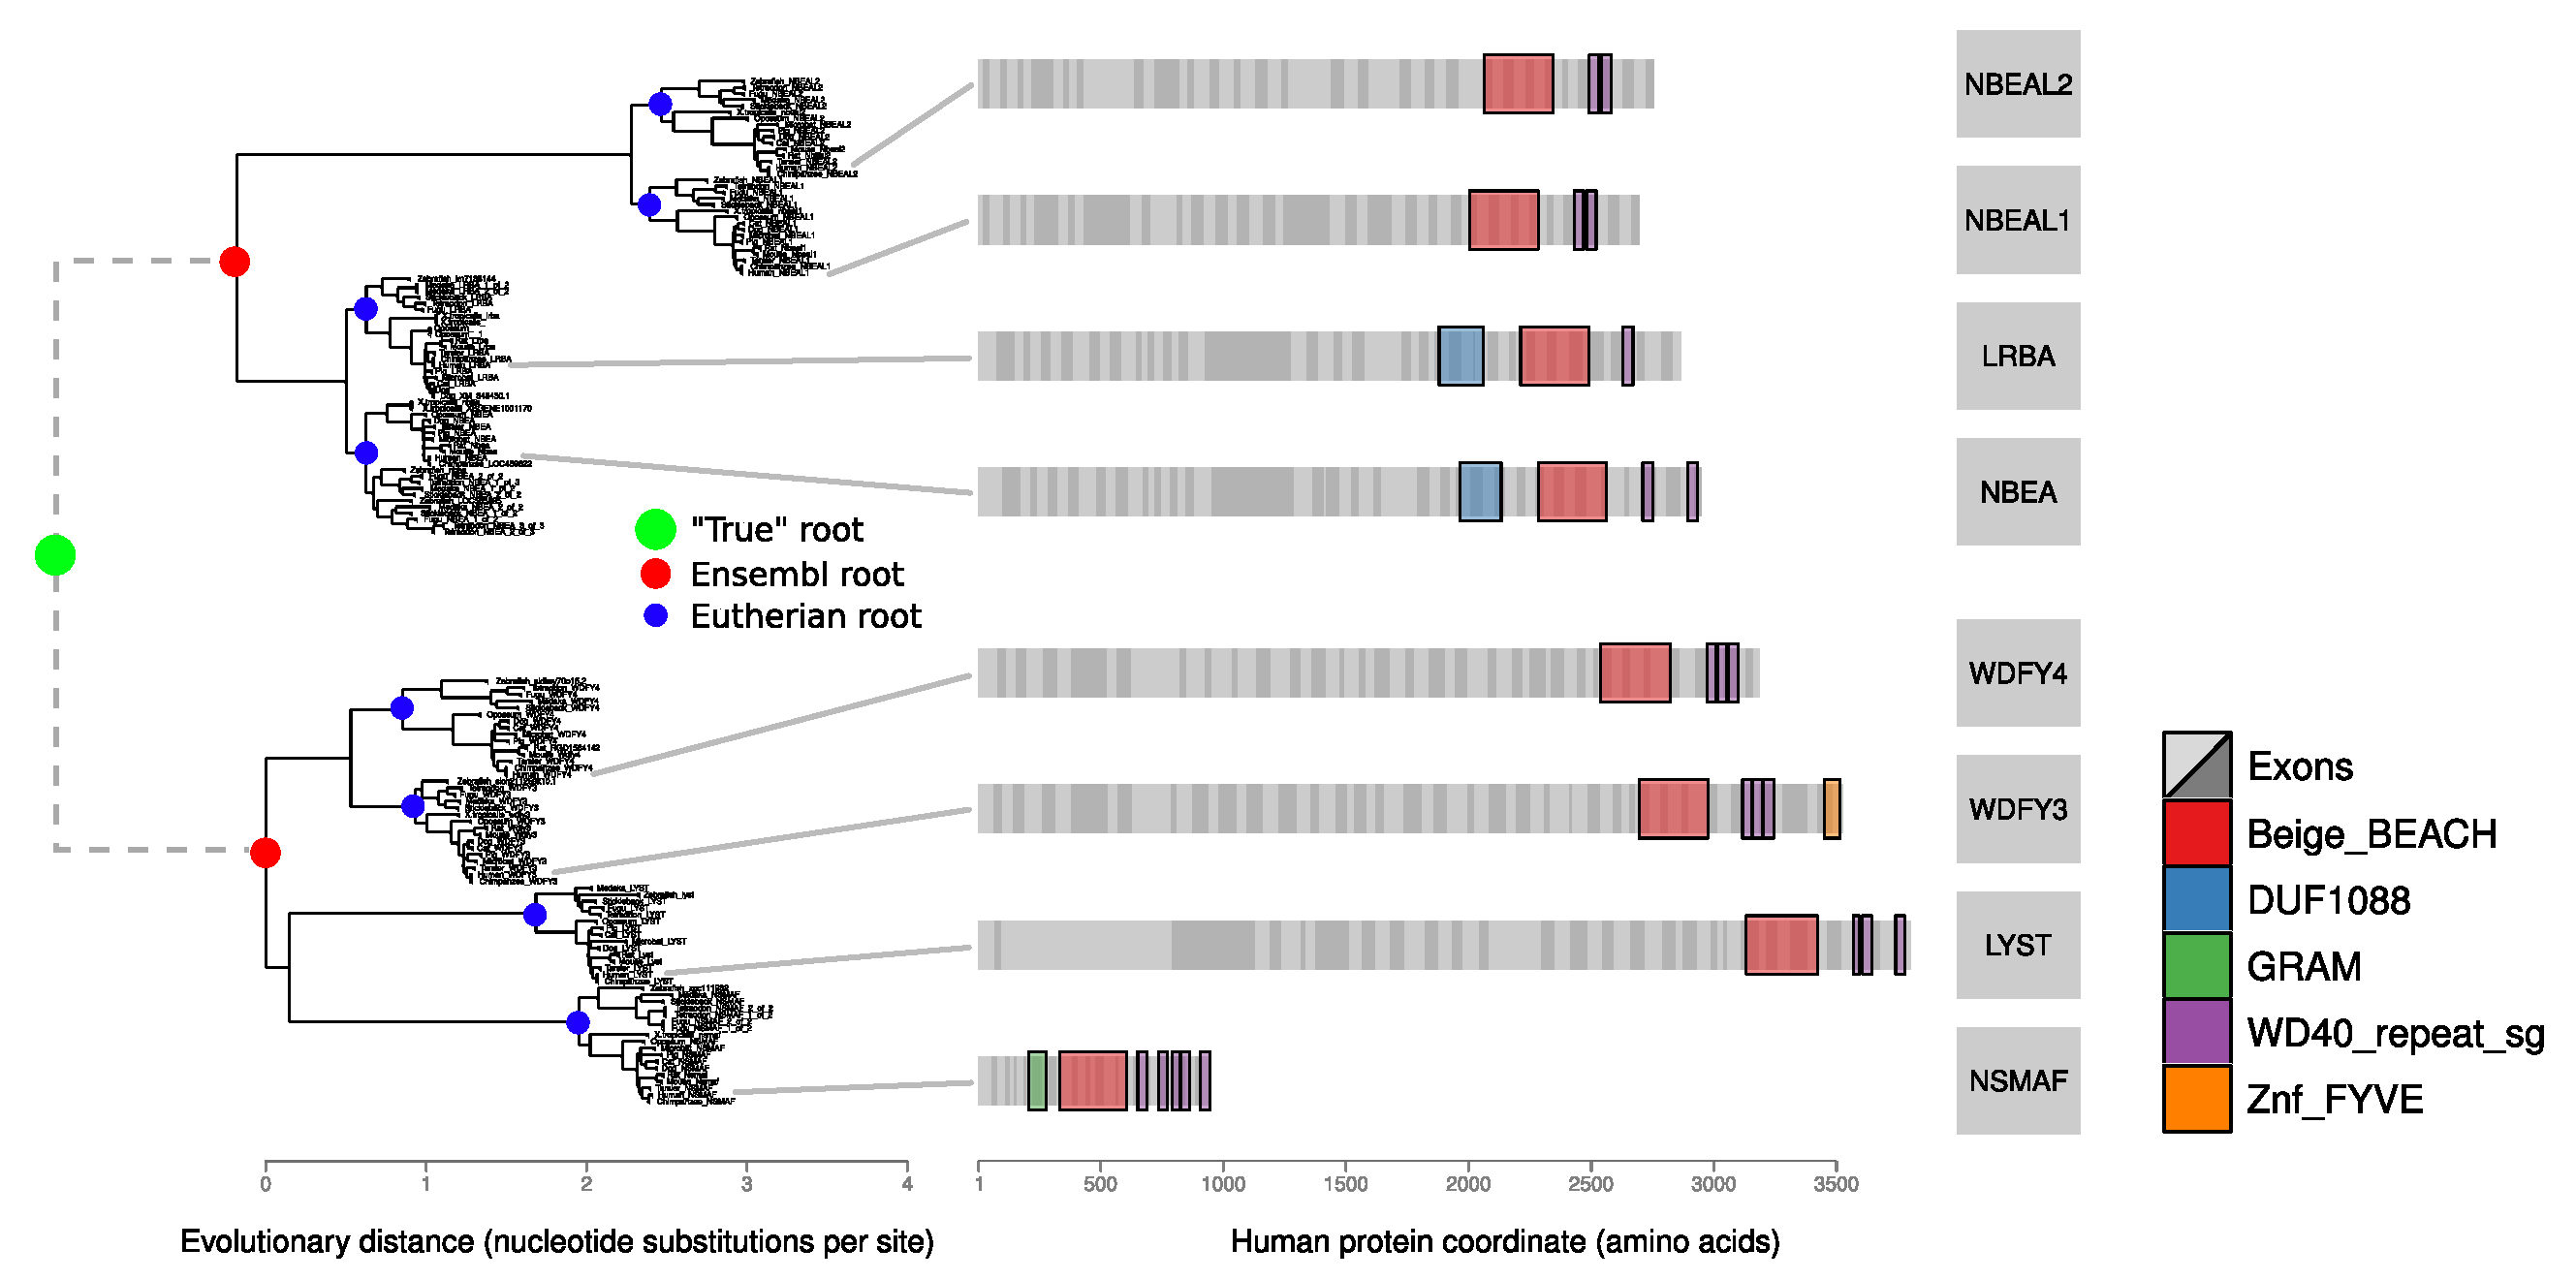
\includegraphics[scale=0.35]{Figs/nbeal2_full.pdf}
\caption{The evolutionary history of the human \gene{neurobeachin-like
    2} gene (\gene{NBEAL2}) and its paralogs. Left, two phylogenetic
  trees from Ensembl Compara (release 60) are shown, summarizing the
  evolution of \gene{NBEAL2} and its three paralogs (top), and
  \gene{LYST}, a presumed distant paralog of \gene{NBEAL2}, and its
  three paralogs (bottom) in 15 vertebrate species. The phylogeny
  shows that \gene{NBEAL2} is taxonomically conserved and distinct
  from its paralogs. Red dots highlight the root nodes of Ensembl gene
  trees, blue dots highlight the root nodes of \euth orthologous
  subtrees, and a dashed line with a green dot represents the putative
  paralogous relationship (with a hypothetical root) between the two
  Ensembl gene trees. Right, the exon and domain structure of each
  human gene is shown: exons are displayed alternating shades of gray,
  and Pfam domain annotations are colored according to their Pfam
  identifier. Adapted from \citep{Albers2011}}
\label{nbeal2}
\end{figure}

As an example, take the gene \gene{NBEAL2} and its human paralogs,
whose gene trees, exon structures and domain classifications were
extracted from Ensembl v62 and summarized in Figure \ref{nbeal2}. A
recent medical sequencing project identified \gene{NBEAL2}, a gene of
previously unknown function, as the putative causative gene for gray
platelet syndrome, a predominantly recessive platelet disorder
resulting in moderate to severe bleeding \citep{Albers2011}. With
Botond Sipos, I performed the evolutionary analysis of \gene{NBEAL2}
for the paper describing the discovery, and it was important for the
purpose of this study to ensure that the \gene{NBEAL2} gene was both
well-conserved across mammals and distinct from its paralogs. The \cmp
pipeline clustered \gene{NBEAL2} with three of its closest paralogs
(\gene{NBEAL1}, \gene{LRBA}, and \gene{NBEA}) into one tree and
similarly clustered four more distant \gene{NBEAL2} paralogs
(\gene{WDFY4}, \gene{WDFY3}, \gene{LYST} and \gene{NSMAF}) into a
separate tree, yielding two views which together showed both the full
taxonomic coverage of the \gene{NBEAL2} \subtr{} and the large amount
of evolutionary distance between paralogs. Had each \mammln ortholog
been displayed independently in \ens (i.e., using the blue ``\euth
root'' nodes in Figure \ref{nbeal2}), it would have been more
difficult for a non-expert to make such claims regarding the
evolutionary history of \gene{NBEAL2} without further
analysis. Conversely, had the \cmp pipeline been even more inclusive
in its clustering approach and identified the hypothetical deeper root
connecting these two sets of trees (represented by the green node in
Figure \ref{nbeal2}), the connection between these eight genes would
have been even more immediately apparent.

%For the purposes of this project, however, it was important to isolate
%individual \mammln gene trees for further processing and sitewise
%analysis. To this end, I designed a simple scheme for splitting gene
%trees into non-overlapping subtrees based on flexible \acl{tc}
%criteria; the remainder of this chapter presentes design and results
%of this process when applied to the \cmp gene trees.

\section[Using taxonomic coverage to extract largely orthologous \mammln \subtr{}s]{Using taxonomic coverage to extract largely \\ \mbox{orthologous} \mammln \subtr{}s}

Based on the observation that the clustering step of the \cmp pipeline
did not make use of any taxonomic information, I hypothesized that a
relatively simple set of rules based on \ac{tc} would be sufficient to
identify most \mammln \acp{lot}. Two well-established observations in
\mammln genomes supported the decision to use \ac{tc} in this
context. First, the existence of two rounds of whole-genome
duplication preceding the evolution of vertebrates \citep{Dehal2005}
suggested that many of the ancient duplication events contained within
Ensembl gene trees occurred before the divergence of \mamml{}s, making
it possible to cleanly separate out taxonomically complete \mammln
\subtr{}s in the majority of cases. This would not be possible if
duplication events were common and spread evenly throughout the
\mammln tree; in that case, many duplication events would have
occurred after the divergence of some or all of the major \mammln
groups, resulting in a larger proportion of \mammln genes with
``internal'' duplications and, thus, fewer singly orthologous trees
with high taxonomic coverage. Second, the overall low rate of gene
duplication and loss in mammals \citep{Demuth2006} (excluding, of the
aforementioned whole-genome duplication events which occurred in the
ancestral vertebrate genome) predicts that few \mammln gene trees will
be subject to one or more gene duplication or loss events. In other
words, most \mammln gene trees should contain sequences from a
majority of \mammln species, so the effectiveness of using \ac{tc} to
identify \mammln \subtr{}s should be largely unaffected by continued
(i.e., post whole-genome duplication) gene duplication or loss
events. The potential utility of \ac{tc} was further bolstered by the
relatively star-like shape of the \mammln tree
\citep{BinindaEmonds2007}: a star-like tree contains more branch
length within terminal lineages than a ladder-like tree with an
equivalent total branch length, making it less likely that a gene
duplication or loss event (if such events occurred randomly throughout
the \mammln tree) would result in a significant disruption to the
\ac{tc} of the gene tree.

To test the validity of this hypothesis, I tested the application of a
variety of alternative \ac{tc}-based methods for extracting \ac{lot}
from the set of \cmp gene trees. I compared these trees to the set of
``root'' \cmp trees and to trees built using homology annotations from
the \ens homology pipeline, with the goal of identifying the most
appropriate set of \acp{lot} to select for further analysis.

The \ac{tc}-based tree splitting process worked as follows. For every
internal node $N$ of each \cmp gene tree, the \ac{tc} was calculated
for several vertebrate clades. The clades examined, and their
associated \acp{tcc} used for the tree splitting process, are shown in
Table \ref{table_subtree_constraints}. The \ac{tc} for node $N$ and
clade $C$ was calculated as $TC(N,C) = species(N) / species(C) $,
where $species(N)$ is the number of unique species represented by the
sequences beneath node $N$ and $species(C)$ is the number of species
within the vertebrate clade $C$. The tree was then evaluated at each
node from root to tip: if a given set of \acp{tcc} were satisfied by
both \subtr{}s below node $N$, then the tree was split into two
\subtr{}s at node $N$, with the new trees having root nodes placed at
the two child nodes, $N_a$ and $N_b$. The process of evaluating and
splitting nodes continued recursively until every node was tested
against the \acp{tcc}. The smallest \subtr{}s which satisfied the
\acp{tcc} were thus included in the resulting \subtr{} set. If only
the entire gene tree satisfied the \acp{tcc} then the entire tree was
included; if the entire gene tree failed to satisfy the \acp{tcc}, it
was excluded altogether from the resulting \subtr{} set.

I chose a variety of clades and \acp{tcc} to evaluate against the set
of \cmp trees, all of which were run against the 18,607 ``root'' trees
within the Compara database to generate several genome-wide \subtr
sets. Table \ref{table_subtree_constraints} shows the details of the
chosen clades and the \acp{tcc} used for each clade. The clade names
(e.g., $TC(Primates)$) refer to the set of species in the \ens
database that are contained within the given \subtr of the NCBI
taxonomy; the NCBI classification of species contained within \ens is
shown in Figure \ref{fig_ncbi_tree}, including labels on the internal
nodes or on the right hand side corresponding to the clade names given
in Table \ref{table_subtree_constraints}.

\begin{figure}
\centering
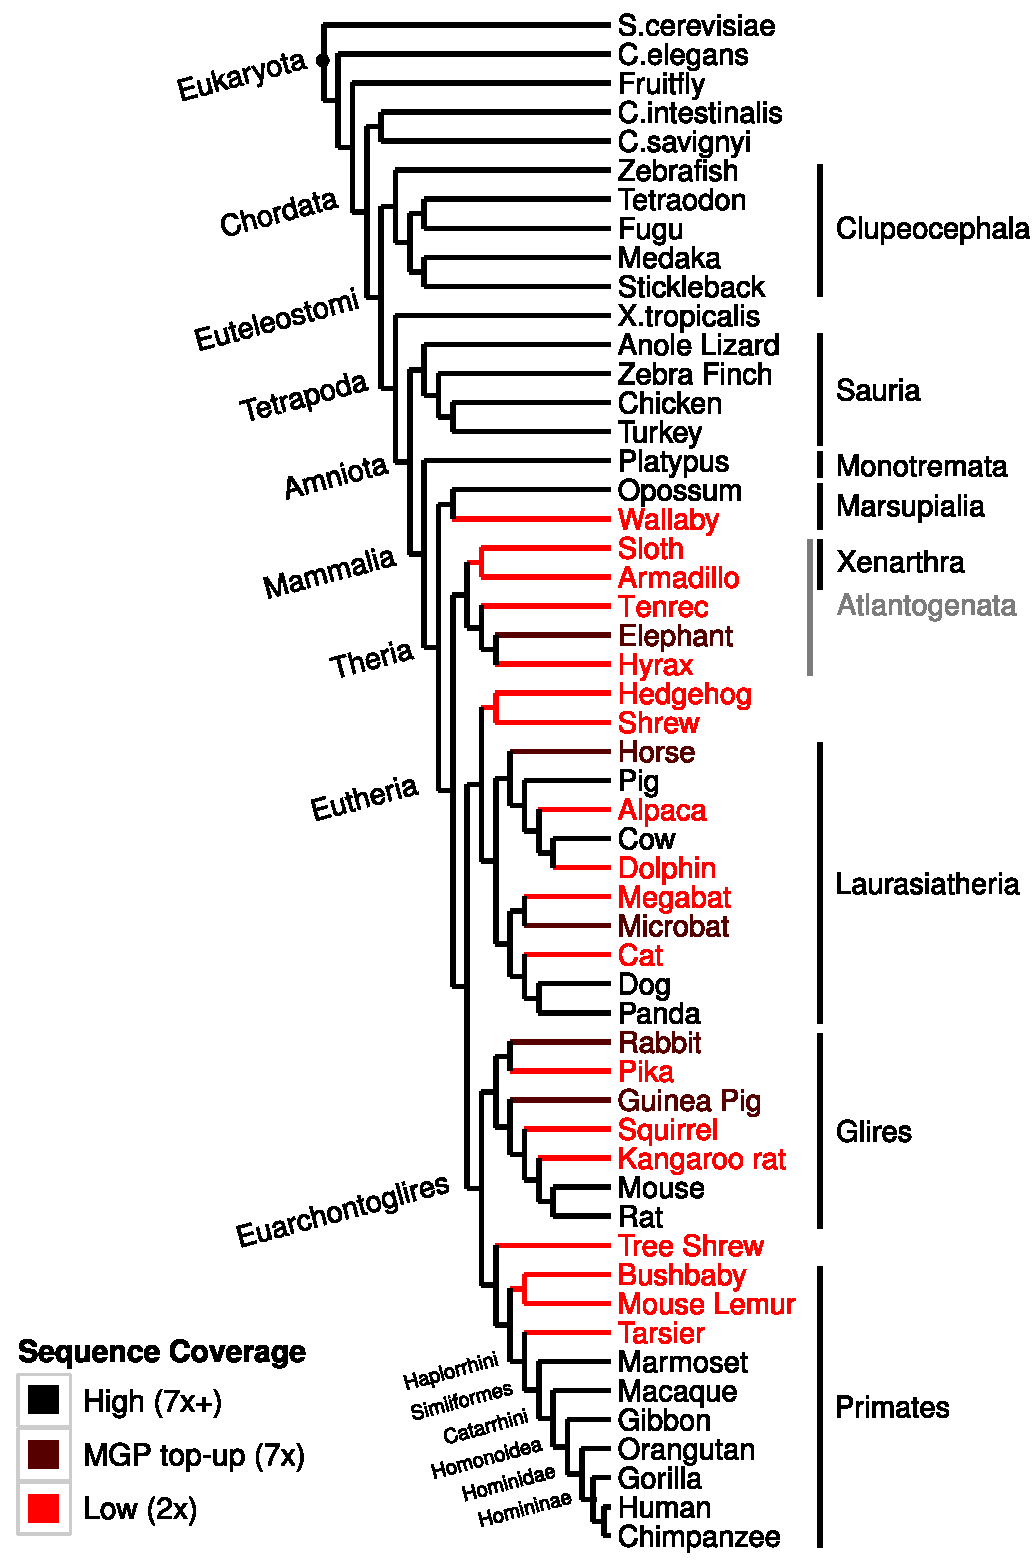
\includegraphics[scale=0.7]{Figs/species_tree.pdf}
\caption{The NCBI taxonomy of species within the Ensembl Compara
  database. Note that branch lengths are not drawn to
  scale. Low-coverage genomes (e.g., those with 2-6x mean sequence
  coverage) are labeled in red, and high-coverage genomes are in
  black. Clade names are included on the left and on the right side of
  the tree.}
\label{fig_ncbi_tree}
\end{figure}

For the Ingroup and Outgroup categories of \acp{tcc}, a \ac{tc} value
of greater than 0.6 was required for a single taxonomic clade. This
value was not arbitrarily chosen; rather, it was important to use a
\ac{tc} value slightly above 0.5 to achieve the desired result of
identifying orthologous \subtr{}s. A value much higher would be too
restrictive: if, for example, the required \ac{tc} value were set to
1, then all subtrees containing a deletion in any species within the
clade of interest would not satisfy the \ac{tcc}. On the other hand, a
required \ac{tc} value of less than 0.5 would allow a single \ac{lot}
to be split into two \subtr{}s, with one \subtr having \ac{tc}$<0.5$,
and the other \subtr, containing the other half of the species within
the clade of interest, also having \ac{tc}$<0.5$. Thus, 0.6 was deemed
a sufficient \ac{tc} requirement for isolating \subtr{}s with
reasonably high \ac{tc} while allowing for some amount of gene
deletion.

Two additional types of \acp{tcc} were designed for use in the
MammalSubgroups and MammalSubgroupsPlusOutgoup methods. Inspired by
the alignment filtering method from Pollard et
al. \citeyearpar{Pollard2010}, which required at least one sequence to
be present from each of the three major mammalian superorders
(Primates, Glires, and Laurasiatheria) for a column to pass through
the filter, the $TC_{min}$ constraint required that the \ac{tc} for all
of the included clades was above a given minimum value. To complement
the $TC_{min}$ constraint, the $TC_{max}$ constraint required that at
least one of the included clades had a \ac{tc} above a given
value. These more complicated \acp{tcc} were included in the analysis
in order to determine whether combinations of more specialized
constraints would perform as well or better than the simplest approach
at isolating \acp{lot} from the \cmp gene trees.

The methods within the Orthologs category of \subtr{} sets were
implemented separately from the rest. Instead of splitting \cmp trees
based on \acp{tcc}, \subtr{}s in the Orthologs category were defined
from the set of genes annotated by the \ens homology database as
orthologs to each gene from a given source species. Thus, for each
gene from the source species, the \cmp \subtr containing all
\ens{}-annotated orthologs was extracted and stored; this was
guaranteed to yield exactly one \subtr{} for every gene in the source
species. This method was tested using human, mouse, zebrafish, and
drosophila as source species.

In contrast to the tree-splitting strategy, the ortholog-based
approach made use of the orthology annotations resulting from \ens{}'s
orthology pipeline.  This pipeline uses the \cmp gene trees as its
source, applying a set of rules to each tree to classify the
relationships between pairs of genes (e.g., one-to-one orthology,
one-to-many orthology, paralogy, etc.). This pairwise approach
implicitly uses taxonomic information when classifying gene
relationships, allowing one to avoid the inclusion of paralogous
genes. The main drawback of this approach was that it was based on
annotations of orthology with respect to a single reference
species. Unless only strict one-to-one orthology was required---which
would have been overly conservative, given the large number of species
included here---the use of a reference species resulted in each
\subtr{} not necessarily containing a completely unique set of
genes. For example, a gene which was recently duplicated in the human
terminal lineage would yield two \subtr{}s, one for each human
paralog, with identical sets of non-human genes in each tree. If those
non-human genes evolved with a large amount of positive selection,
then this signal would over-represented in the downstream analysis due
to the inclusion of multiple copies of those sequences. The tree-based
\subtr splitting approach was preferable in this regard, guaranteeing
that each \ac{lot} would only be included once in the analysis. Still,
I expected that the sets of \subtr{}s resulting from the \ens ortholog
annotations would serve as a useful reference against which to compare
the methods based purely on \acp{tcc}.

\begin{table} \footnotesize
\centering
\begin{tabular}{@{}lll@{}} \toprule
\multicolumn{2}{c}{Method} \\ \cmidrule(r){1-2}
   Category & Name & Constraints \\ \midrule
Ingroup & Primates & $TC(Primates) > 0.6$ \\
 &   Glires &  $TC(Glires) > 0.6$ \\
 &   Laurasiatheria & $TC(Laurasiatheria) > 0.6$ \\
 &   Sauria & $TC(Sauria) > 0.6$ \\
 &   Fish & $TC(Clupeocephala) > 0.6$ \\
Outgroup &  Eutheria & $TC(Eutheria) > 0.6$ \\
 &   Amniotes & $TC(Amniota) > 0.6$\\
 &   Vertebrates & $TC(Vertebrata) > 0.6$\\
 &   Fungi/Metazoa & $TC(Fungi/Metazoa) > 0.6$\\
Subgroups &  MammalSubgroups & $TC_{min}(Laur., Glires, Primates) > 0.1$\\
 &   \scriptsize{MammalSubgroupsPlusOutgroup} & $TC_{min}(Laur., Glires, Primates) > 0.1$ AND \\
 &    & $TC_{max}(Sauria, Clupeo., Ciona, Marsup.) > 0)$ \\
Orthologs & Human Orthologs & \\
 &   Mouse Orthologs &  \\
 &   Zebrafish Orthologs &  \\
 &   Drosophila Orthologs &  \\
Root Nodes & Ensembl Roots &  \\
\bottomrule
\end{tabular}
\caption{Subtree constraints used for identifying \euth
  orthologous subtrees. Ensembl gene trees were split into subtrees
  based on \acf{tc} requirements at internal
  nodes. Laur.---Laurasiatheria; Clupeo.---Clupeocephala; Marsup.---
  Marsupiala.}
\label{table_subtree_constraints}
\end{table}

The \subtr{} splitting scheme was applied to the 18,607 gene trees
from the \cmp database, producing a set of \subtr{}s for each of the
\acp{tcc} shown in Table \ref{table_subtree_constraints}. In the next two
sections I will describe the resulting sets of trees and \subtr{}s and
discuss what they reveal about the evolutionary history of vertebrates
and the feasibility of using \acp{tcc} to isolate \mammln \acp{lot} for
sitewise analysis.

\section{Analysis of the set of root Compara gene trees}
\label{section_root_compara_trees}

Table \ref{table_ensembl_roots} presents a summary of the set of root
Compara gene trees and the subsets of trees with greater or fewer than
15 sequences. The ``root'' gene trees are the set of 18,607 gene trees
contained within the \ens \cmp database.

A first observation was that, somewhat surprisingly, nearly half of
all \cmp gene trees contained few sequences: 9,378 out of 18,607 root
trees constituted fewer than 15 sequences. Given the protein-based
clustering performed by the Compara pipeline, one might expect many of
these small trees to represent portions of larger fast-evolving gene
trees whose high sequence divergences made the BLAST search step
inaccurate or caused clustering via the \hclust algorithm to be
ineffective. Alternatively, these small gene trees might have resulted
from extensive gene loss, lineage-specific gene duplications or from
pseudogenes being mis-annotated as genes. In the case of
lineage-specific duplications or pseudogene mis-annotation, tight
clusters of very closely-related transcripts would have been
identified by \hclust as independent clusters of homologs. Some
evidence for the latter scenario could be found in the median species
counts and mean path lengths of the smaller (fewer than 15 sequences)
versus larger (greater than 15 sequences) trees, shown in the second
and third rows of Table \ref{table_ensembl_roots}. The set of small
root trees had a median species count of 2, compared to 47 for the
large trees, indicating that the smaller trees encompassed sequences
from very small taxonomic ranges. I also calculated the \ac{mpl} of
each tree, defined as the mean root-to-tip path length of all lineages
in the tree, to assess the amount of sequence divergence contained
within each tree. The median \ac{mpl} for small trees was 0.04
compared to 1.04 for the large subset, revealing much lower amounts of
sequence divergence within each tree. These two summary statistics
together provided evidence that the smallest gene trees in the \cmp
database consist of highly species-specific, closely-related proteins;
it was likely that many of these small trees represented artifactual
gene annotations and should be removed prior to any downstream
analysis.

Despite the existence of many small gene trees in the \cmp database,
they together comprised only a small fraction of all protein-coding
sequences. Only 809 human genes, or 4\% of the total human gene
set---a gene set which I expected be well-annotated and to contain few
false positive genes due to the high level of manual curation and the
large amount of continued scrutiny---was contained within the subset
of small trees. This indicated that whatever process was causing the
\cmp pipeline to yield a high number of small gene trees did not have
much of an impact on the overall placement of human protein-coding
genes within the database of root \cmp gene trees.

As mentioned in Section \ref{section_quantifying_paralogous}, a closer
examination of the distribution of tree sizes in the set of root \cmp
trees presented a clear view of the over-clustering of \mammln
\acp{lot}. The black bars in Figure \ref{fig_ensembl_roots_hist} show the
distribution of sequence counts for all trees with more than 15
sequences, with vertical dashed lines overlaid at multiples of 48, the
number of vertebrate species in \ens release 63. The highest peak of
the histogram is at or slightly above 48 sequences, with the tree
counts quickly diminishing at larger sizes. Weaker, but still
discernable, peaks exist at larger tree sizes, with the location of
these wave-shaped peaks corresponding closely to the second, third and
fourth multiples of 48. The pattern of recurring peaks is
indistinguishable at sizes above 200, but there is still a long tail
of large trees extending out to a maximum size of 400
sequences. Overall, the distribution of tree sizes provided good
support for the scenario described in Section
\ref{section_quantifying_paralogous}, with the \cmp pipeline often
clustering together two or more \mammln \acp{lot} related by a more
distant duplication event.

It was also informative to characterize the set of root \cmp gene trees by
the proportion of all protein sequences which are covered by trees of
a given size or smaller. This value is plotted in Figure
\ref{fig_ensembl_roots_hist} as a gray line. First, this plot showed
that trees with fewer than 15 sequences (which were excluded from the
plot but included in the calculation of the cumulative distribution
shown) represented a very small fraction of the sequences within the
\cmp database; this observation was similar, but not identical, to the
statistic noted above, that only 4\% of human genes were contained
within small trees. Second, the steady upward slope of the cumulative
curve contrasted with the declining height of the histogram bars at
higher sequence counts. This was a result of the increasing number of
sequences encompassed by each of the larger trees: although relatively
few trees contained more than 300 sequences, together they comprised
around 10\% of all protein-coding genes in \cmp. This cumulative plot
helps identify two other points of particular interest. First, one can
use the height of the cumulative line at the beginning of the second
hump in the histogram (at around 75 sequences) to identify the
fraction of vertebrate proteins which exist in the \cmp database as
members of a duplicated \mammln \ac{lot}. (The trees with between 48
and 75 clearly contained some number of duplicate genes, but these
likely consisted of more recent duplication events as opposed to
ancient duplications leading to entirely separate \acp{lot}.) . The
cumulative line showed that around 30\% of proteins are covered by
trees of 75 sequences or fewer, meaning that 70\% of vertebrate
proteins are contained within large gene trees containing
sequence-based evidence of ancient paralogy. Second, using the
cumulative line in the reverse direction identifies the tree size
above which 50\% of all sequences were clustered. This value
represents the size of tree that an ``average'' protein might be
clustered in, and in some ways is a more accurate characterization of
a set of gene trees than the median tree size. A similar calculation
is often performed to characterize the size distribution of contiguous
sequence blocks (contigs) within a genome assembly. This statistic,
referred to as the N50 length, is the contig length for which 50\% of
bases are contained in contigs of that size or larger
\citep{Miller2010}. For the \cmp gene trees, the N50 tree size was
139, slightly less than three times the number of vertebrate species
(Table \ref{table_ensembl_roots}). Thus, the average protein in the
set of \cmp gene trees belonged to a tree with 139 sequences,
corresponding roughly to three \mammln \acp{lot} related by ancient
duplication events, likely resulting from the two rounds of vertebrate
genome duplication.

\bbfig
\centering
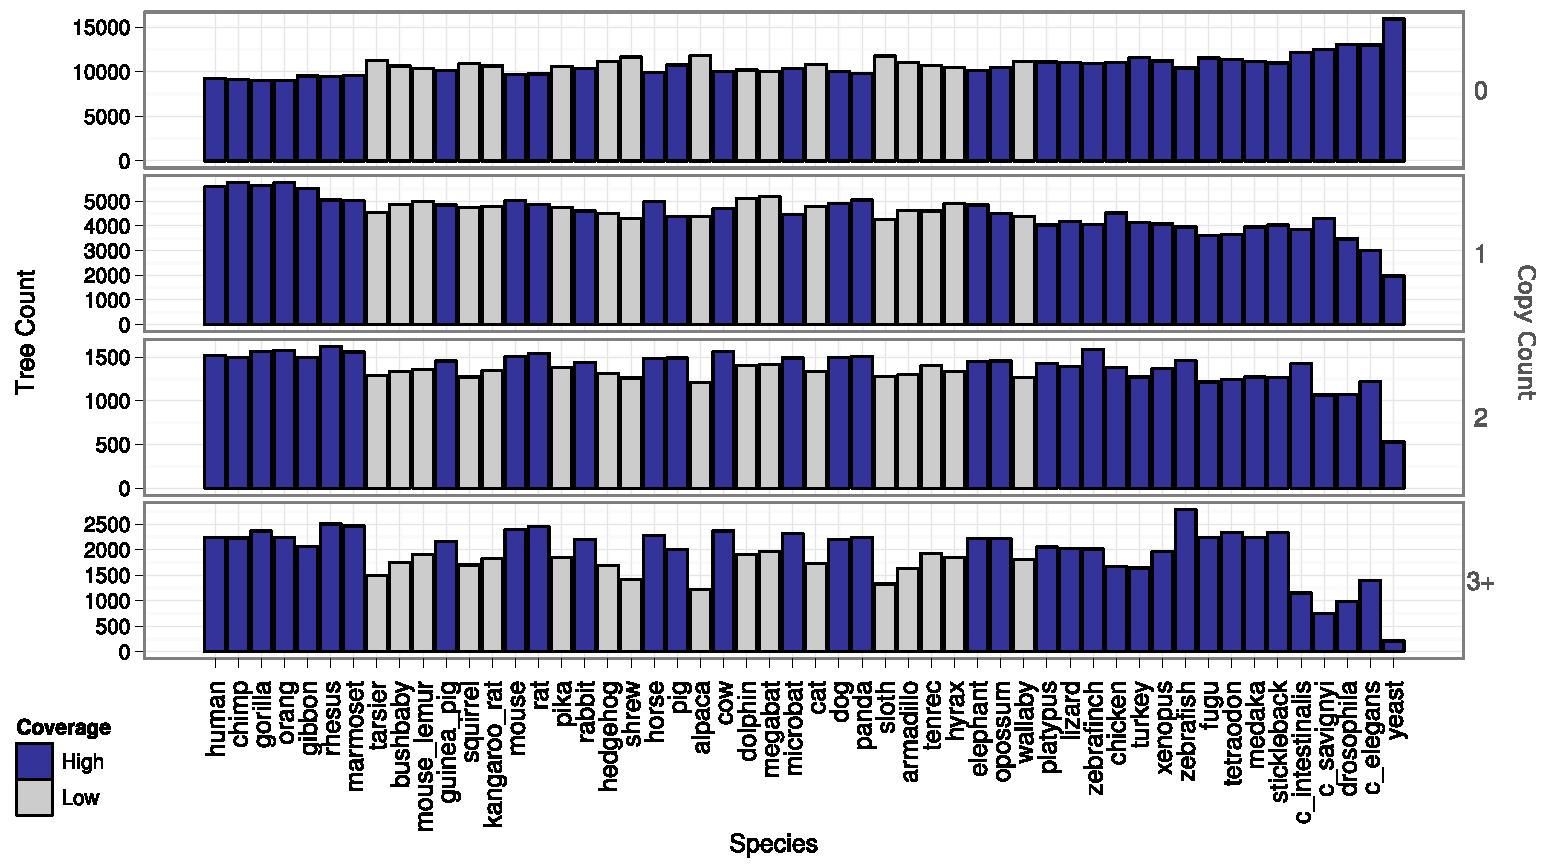
\includegraphics[scale=0.83]{Figs/dups_ens_roots.pdf}
\caption{Taxonomic distribution of gene copy counts for the ``root''
  Ensembl trees. The number of trees containing 0, 1, 2 or more than 3
  sequences from each species is shown. Bars are colored blue and gray
  for species with high- and low-coverage genomes, respectively. Note
  that the y-axis scale is not the same for each panel.}
\label{ortholog_root_dups}
\eefig

Another way to characterize the distribution of \cmp gene trees was
across the taxonomic space. Given the wide range of quality in genome
assemblies and annotation sets contained within \ens, a question of
particular interest was whether levels of gene presence and absence
were consistent across different species groups and different levels
of assembly quality. To investigate this question in the context of
the root \cmp gene trees, data were collected by counting the number
of sequences from each species contained within each gene
tree. Results of this analysis are presented in Figure
\ref{ortholog_root_dups}, showing the number of trees containing 0, 1,
2, or more than 3 genes from each of the 53 species within \ens (note
that the total of 53 species includes 38 mammals, 10 non-mammalian
vertebrates, and 5 non-vertebrates). Comparing the ranges of values
for each copy count (labeled 0, 1, 2 and 3+), I found that the largest
number of trees contained zero copies from any one species (between
8,000--11,000 within vertebrate species), a smaller but large number
of trees contained one copy from a species (between 4,000-6,000) and
several thousand trees contained two, three or more copies (between
1,000-1,500 for 2 copies and 1,500-2,000 for 3+). Note that these
numbers were tabulated independently between species; for example, the
10,000 \zcop trees in human were counted independently of the 10,000
\zcop trees in chimpanzee, so nothing could be said about how many
trees contained zero copies in both human \emph{and} chimpanzee. As
noted in the analysis of tree sizes, the large number of \zcop trees
reflected the large number of small, species-specific trees within the
set of \cmp gene trees. Similarly, the large number of trees with many
copies from each species reflected the trees with multiple \mammln
\acp{lot} clustered together.

Comparing numbers horizontally across the range of species in Figure
\ref{ortholog_root_dups} revealed that the zero-copy count tended to
increase with increased evolutionary distance from human, while the 1,
2 and 3+ copy counts tended to decrease as the distance from human
increased. Both trends were most striking at the distant end of the
tree, where the five non-vertebrate species are shown. For the
increase in \zcop trees and the decrease in single-copy trees, the
strength of the trend at the highest level of divergence can be partly
explained by the long branch lengths connecting those species to each
other and to the more densely sampled vertebrate clade: the
distance-based clustering algorithm might reasonably be expected to
produce more false negatives in longer branches for a number of
reasons, including the behavior of the \hclust algorithm, inaccurate
BLAST E-values at large distances, and heterogeneity in evolutionary
rates across lineages \citep{Whelan2008}. However, the reduced numbers
of 2 and 3+ copy count trees in non-vertebrate species were most
likely due to the whole-genome duplications at the basal vertebrate
lineage, resulting in the non-vertebrate species (which did not share
in the vertebrate-specific genome duplications), being strongly
depleted of multi-copy duplicates compared to their vertebrate
relatives. Some of this pattern may be attributable to a bias in \ens
towards vertebrate genes, as the yeast \emph{Saccharomyces cerevisiae}
underwent a separate lineage-specific genome duplication event
\citep{Kellis2004} but contains few multi-copy genes in the set of
\cmp trees.

Knowing that many of the \lcv genomes were annotated using projections
based on the human set of transcripts, it was slightly concerning that
human and its close primate relatives contained fewer zero-copy genes
and more 1-copy and 2-copy genes than any other group of vertebrates
in the \cmp set of trees. There was no \emph{ab initio} biological
reason to expect this to be the case, so I suspect that this pattern,
which was fairly small in effect, was due to the widespread reliance
on human annotation and protein experimental data in the annotation of
non-human genomes. Although most of Figure \ref{ortholog_root_dups}
follows the patterns described above, one interesting deviation was
found in the 3+ copy count for the fish species. Whereas the 5 fish
species had noticeably fewer 1- and 2-copy genes than primates, the
number of trees with 3+ copy counts in fish species was roughly equal
to or greater than those for human or any primates. This was most
likely a result of gene duplicates retained after the third round of
genome duplication in the teleost ancestor \citep{Jaillon2004}. The
signal resulting from the teleost genome duplication event was clearer
in the set of \subtr{}s identified using the Fish set of \ac{tcc} (see
Table \ref{table_subtree_constraints}), so I will defer further
discussion of this effect to Section
\ref{section_analysis_sets_subtrees} where that set of trees is
described.

Finally, the differences in copy counts between species with low- and
high-coverage genome sequences showed the tendency of \lcv genome
sequences to be absent from gene trees or to show reduced copy
counts. Low-coverage species contained more \zcop, roughly the same
number of 1-copy, and noticeably fewer multi-copy genes compared to
closely-related high-coverage species. These clear differences showed
that gene absence in \lcv genomes should not be taken as evidence for
actual gene loss, and that multi-copy genes are systematically
underrepresented in \lcv genomes. The former point was emphasized in a
recent critical analysis of the impact of \lcv genomes on gene
duplication inference in the \cmp database \citep{Milinkovitch2010},
but the latter point was largely ignored. Again, this signal was also
stronger in the sets of \ac{tc}-defined \mammln \subtr{}s and will be
revisited in the next section.

The preceding analysis of the set of root \cmp gene trees, in which I
characterized the distribution of trees with respect to size and
across the taxonomic space, showed that despite the
over-representation of small, species-specific trees, most sequences
were contained in trees with biologically plausible sizes given the
history of vertebrate whole-genome duplications. A gene tree-based
equivalent of the N50 statistic was developed for summarizing the
distribution of protein sequences within differently-sized gene trees,
and two visual summaries of this distribution were introduced (in
Figures \ref{ortholog_root_dups} and \ref{fig_ensembl_roots_hist}),
providing evidence for the clustering of paralogous mammalian
sub-trees and for species-based and genome quality-based trends in the
breakdown of gene copy counts within the root \cmp gene trees.

\section{Analysis of sets of \subtr{}s defined by taxonomic coverage and orthology annotation}
\label{section_analysis_sets_subtrees}

The sets of trees resulting from applying the \subtr splitting scheme
with various \acp{tcc} to the \cmp gene trees are summarised in Table
\ref{ensembl_subtree_table}, with a summary of the root \cmp gene
trees and a summary of the set of seven-species amniote gene trees
from the OPTIC database \citep{Heger2008} included at the bottom for
comparison.


\bbtable
\centering \footnotesize
\begin{tabular}{llrb{2.5cm}rrrrrrrr}
\toprule

\multicolumn{2}{c}{Subtree Method} & Tree & \multicolumn{3}{c}{Sequence Counts} & \multicolumn{3}{c}{Human Content} & Human & Med. & Med. \\ 
\cmidrule(r){1-2} \cmidrule(r){4-6} \cmidrule(r){7-9}
Category & Name & Count  & \scriptsize{Med (Min / Max)} & Total & N50 & 0 & 1 & 2+ & Total & MPL & Species \\ 

%\multicolumn{2}{c}{Subtree Method} & &  Med. Size & &  & \multicolumn{3}{c}{Human Content} & Human & Med. & Med. \\ \cmidrule(r){6-8} \cmidrule(r){1-2}
%Category & Name & Count  & (Min / Max) & Count & N50 & 0 & 1 & 2+ & Total & MPL & Species \\ 
  \midrule
\input{Tables/ortholog_summary.txt}
\bottomrule
\end{tabular}
\caption{Summary of Ensembl \subtr{}s identified using taxonomic
  criteria or Ensembl ortholog annotations. The set of \cmp gene trees
  from Table \ref{table_ensembl_roots} and the set of trees from the
  OPTIC database \citep{Heger2008} are included at the bottom for
  comparison. Cells in numeric columns are shaded according to their
  value relative to other rows, with low values in white and high
  values in blue. The ``Human Content'' columns represent the fraction
  of trees which contain the indicated number of human
  genes. ``Med. Species'' is the median species count across all
  trees. Med.---median; MPL---mean path length.}
\label{ensembl_subtree_table}
\eetable


The Ensembl Roots and Drosophila Orthologs sets were two clear
outliers among the \subtr sets shown in Table
\ref{ensembl_subtree_table}, with much higher N50 values (139 and 125
vs. the next highest value of 56) and more trees with multiple human
copies (0.20 and 0.43 vs. the next highest value of 0.14) than any
other \subtr set. In fact, these two \subtr sets were very similar
except for the excess of small species-limited trees in the Ensembl
Roots set: the Drosophila Orthologs set contained fewer trees than the
Ensembl Roots (9,210 vs. 18,607) and a larger average tree size (60
vs. 15), and the summary values closely resembled the set of Ensembl
Roots with small trees removed (Table \ref{ensembl_root_table}). These
methods will thus be ignored in the discussion through the remainder
of this chapter.

The sets of trees resulting from the different Ingroups \ac{tcc}
methods might be expected to show different characteristics if
different groups of species (e.g., fish versus birds or mammals)
experienced different large-scale patterns of gene duplication or gene
loss subsequent to the divergence of their lineages. Given the
well-accepted evidence for a teleost-specific whole genome duplication
\citep{Jaillon2004}, I expected the Fish \ac{tcc} to behave
differently, but less certain was whether there would be significant differences
between the trees resulting from Sauria or the 3 mammalian \ac{tcc}.

The 3 methods based on mammalian \acp{tcc} (Primates, Glires and
Laurasiatheria) produced largely similar sets of trees, with the
Primates set containing around 2,000 more trees and covering around
1,000 more human genes than the Glires and Laurasiatheria sets. There
was no readily apparent reason for the higher number and human gene
coverage of Primate trees, although it may be due to an excess of
primate-specific gene trees that were not captured by non-primate
\acp{tcc}.

The Sauria set of \subtr{}s was noticeably different from the
mammal-based \acp{tcc} sets from the Ingroups category. The Sauria
clade was represented by only four species in Ensembl and diverged
from the \mammln ancestral population at an early point in the
evolution of amniotes (Figure \ref{fig_ncbi_tree}); it is plausible
that the lower clade size and long branch length separating Sauria
from the other vertebrate clades caused the moderately lower number of
trees (13,046 vs. 15,764 for Laurasiatheria) and the increased
proportion of trees containing multiple human genes (0.14 vs. 0.09 for
Laurasiatheria).

The Fish clade \ac{tcc} produced a strikingly different set of trees,
resulting from the impact of the teleost-specific whole-genome
duplication on the structure of gene trees in fish. Although the Fish
\subtr set yielded a N50 value of 49, which was no different from the
N50 of the other Ingroups sets, Table \ref{ensembl_subtree_table}
highlights three major differences in the Fish set: it contained many
more trees, a higher proportion of trees with zero human copies, and a
lower total human gene count than the other Ingroups sets.

The reason for the drastically different Fish tree set was that the
tree splitting procedure was designed to identify the largest
non-overlapping set of \subtr{}s that satisfied the given
\acp{tcc}. Genes where one or both of the duplicate copies from the
teleost-specific whole-genome duplication were lost would appear as
one-to-one orthologs or deletions with respect to the other vertebrate
lineages. Genes that were retained in duplicate form, however, would
result in a gene tree with two teleost-specific \subtr{}s, each
containing a high \ac{tc} value (i.e., near or equal to 1.0) for the
Clupeocephala clade that contains the fish species within \ens. In
this case, the splitting procedure would produce two small
fish-specific \subtr{}s, ``ignoring'' the surrounding set of mammalian
orthologs because two smaller non-overlapping trees already exceeded
the \ac{tc} threshold of 0.6. If, however, one of the duplicate gene
copies were lost, then the tree would resemble a typical
singly-orthologous vertebrate gene tree, and the splitting procedure
would select a \subtr encompassing the entire vertebrate clade. It
follows that the presence of small, teleost-specific gene trees in the
Fish set is a signal of retained duplicate copies, and the size
distribution of trees from the Fish set, shown in Figure
\ref{ensembl_fish_hist}, shows that several thousand trees fit the
expected model. If we assume that all trees from the Fish subset that
contain no human copies, span 5 or fewer species, and contain 40 or
fewer sequences are likely retained duplicate genes, a total of 6,980
retained duplicates are identified, yielding a retention rate of
17.5\%, which is very much in line with a previously published
estimate of 15\% based on a comparison of tetraodon, fugu and
zebrafish genes \citep{Brunet2006}.

\begin{figure}
\centering
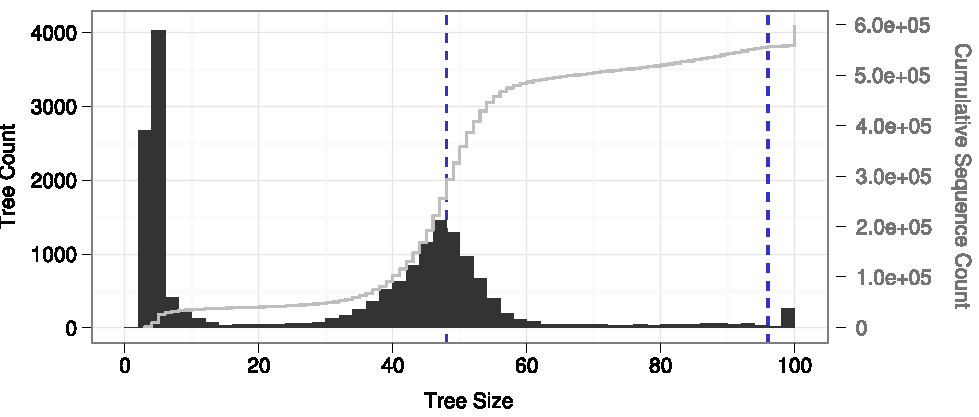
\includegraphics[scale=0.9]{Figs/hist_fish_roots.pdf}
\caption{Tree sizes for the set of \subtr{}s identified using the Fish
  clade taxonomic coverage constraint, showing an excess of small
  \subtr{}s resulting from the teleost genome duplication. Black bars
  show a histogram of tree sizes in bins of width 2, a gray line shows
  the cumulative number of sequences contained within trees of that
  size or smaller, and dashed blue lines are drawn at integral
  multiples of 48, the number of vertebrate species within
  Ensembl. Trees with more than 100 sequences are included in the
  topmost bin.}
\label{ensembl_fish_hist}
\end{figure}

The sets of \subtr{}s resulting from the Outgroup methods were of
special interest, as the clades used to define these \acp{tcc}
contained all or nearly all of the \mammln species whose orthologous
genes I wished to study. The resulting sets of \subtr{}s showed little
variation, owing perhaps to the large sizes of the clades and their
similar species composition. Each \subtr set contained between
15,000--17,000, N50 values of around 49, and greater
than 90\% of trees containing exactly one human sequence. These
measures provided strong evidence that the tree-splitting method was
accurately isolating \mammln \acp{lot}.  Some slight differences
between \subtr sets were apparent, however, with the tree count
decreasing, the proportion of trees with human duplications
increasing, and the overall human gene coverage decreasing as the
clade size used for the \ac{tc} calculation increased. These trends
could potentially be explained by the minimum required tree size
increasing along with the clade size, as a result of the increased
number of species required to produce a \ac{tc} value of 0.6. The
minimum \subtr size ranged from 21 for Eutheria to 32 for
Fungi/Metazoa.

The Subgroups methods did not appear to produce \subtr{}s of any
higher quality or more biological interest than the Outgroups
methods. The MammalsSubgroups set produced more trees than the
Outgoups sets, but the N50 was slightly lower (46 vs. 49) and the
proportion of \zcop human trees was higher (0.18 vs. 0.01), suggesting
that the additional trees in the MammalsSubgroups set were spurious
\subtr{}s containing limited species coverage. The addition of an
outgroup requirement to the \mbox{MammalSubgroupsPlusOutgroup} method
produced a tree set more closely resembling the Outgroup methods, but
the human gene coverage was lower than that for any Outgroup method
despite the overall higher tree count.

Finally, the ortholog annotation-derived \subtr{}s provided for an
interesting comparison between the three different ortholog sources
and between the overlapping and non-overlapping sets of \subtr{}s. The
\species{Drosophila} ortholog set was very different from the
vertebrate sets due to the two rounds of whole genome duplication,
while there was minimal variation among the other ortholog sets. It is
interesting to note that the protein-coding transcripts used by the
\cmp pipeline included 21,873 mouse protein-coding genes and only
19,991 human genes, indicating either a larger number of true
protein-coding genes in mouse or a higher tolerance for false positive
gene predictions in the mouse genome compared to the human
genome. Zebrafish, on the other hand, contained 24,540 genes; this
number agreed well with the 17.5\% proportion of retained duplicate
genes that I estimated earlier in this section. Overall, 76\% and 81\%
of mouse and zebrafish genes contained an apparent orthologous
relationship with one human gene, which was only slightly lower than
the 92\% of Eutheria \subtr{}s containing one human sequence.

\begin{figure}
\centering
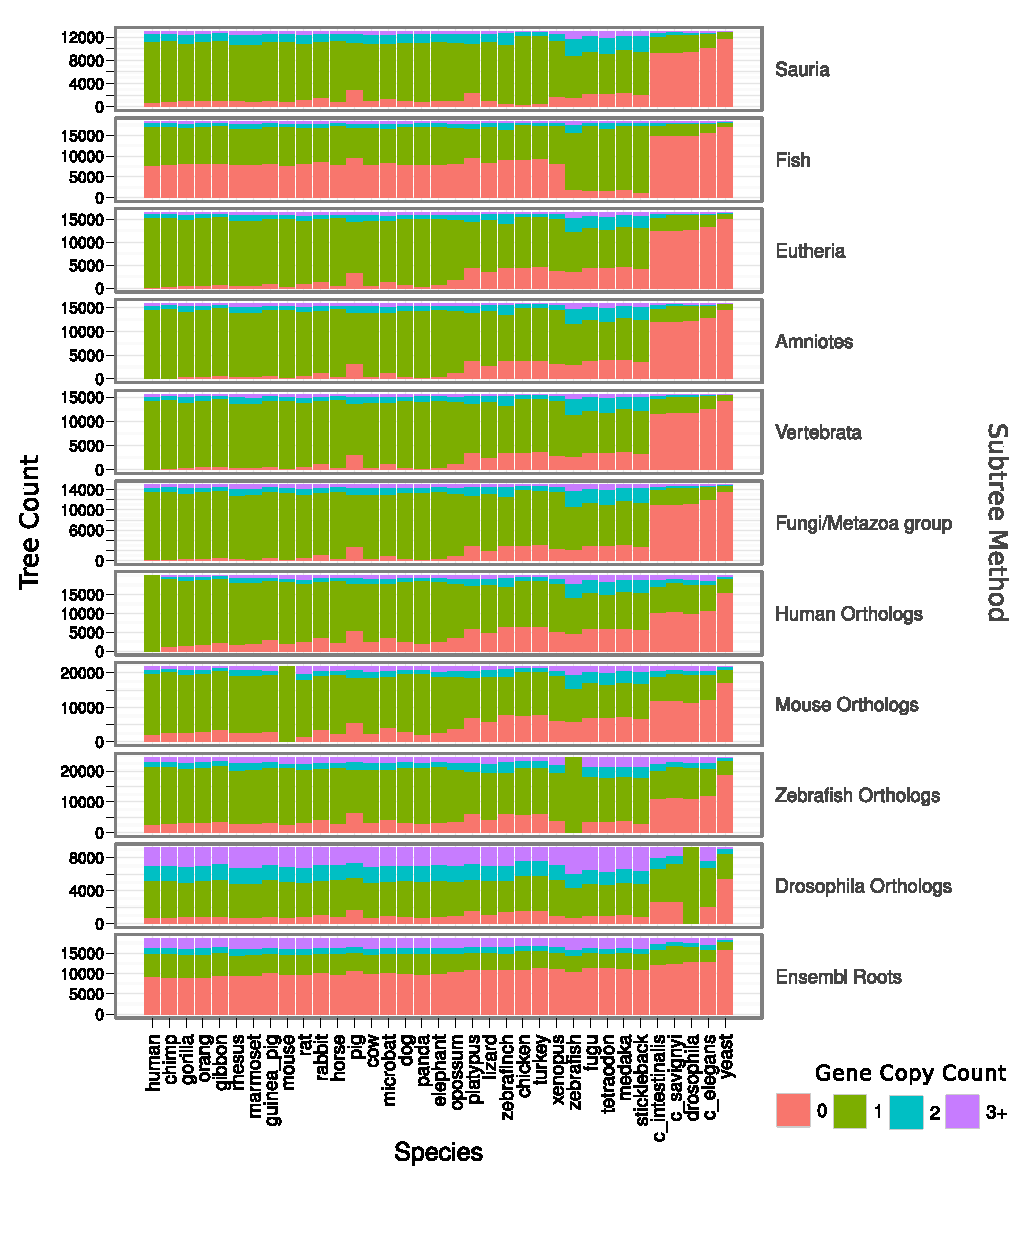
\includegraphics[scale=0.9]{Figs/tax_ens_roots.pdf}
\caption{Taxonomic distribution of gene copy counts for different
  \subtr methods. The numbers of trees containing 0 (red), 1 (green),
  2 (blue) or more than 3 (purple) sequences from each species are
  shown as stacked colored bars. The Ingroup and Subgroups methods
  were omitted for clarity, as were species with low-coverage
  genomes. Note that the y-axis scale is not the same for each panel.}
\label{ortholog_stacked_bar}
\end{figure}


In order to easily compare patterns between \subtr sets and across the
taxonomic space, I tabulated gene copy counts within each \ens species
for each generated \subtr set; the results of this analysis are shown
in Figure \ref{ortholog_stacked_bar}. By way of reference, the values
shown in each of the separate panels of Figure
\ref{ortholog_root_dups} appear in the bottom panel of Figure
\ref{ortholog_stacked_bar} as stacked bars of different
colors. Although the various summary characteristics of each of the
\subtr methods have already been discussed at length, this more
taxonomic-oriented view revealed some salient features of the patterns
of gene deletion and duplication within the tree sets and showed the
pervasive impact of genome-wide duplications on the evolution of
vertebrate genes. The large fraction of species with multiple copies
in the Drosophila Orthologs \subtr set (Figure
\ref{ortholog_stacked_bar}, Drosophila Orthologs, blue and purple
bars) shows the effect of two rounds of vertebrate genome evolution,
producing a large number of trees with multiple Drosophila orthologs
in vertebrate species; similarly, the elevated fraction of multi-copy
fish trees in the Outgroups \subtr sets (e.g., the blue bars in the
Eutheria panel of Figure \ref{ortholog_stacked_bar}) showed the impact
of the teleost-specific duplication event on the number of \mammln{}
\acp{lot} with multiple fish copies.

\section{Gene duplication and loss in the set of Eutherian largely orthologous trees}

The \subtr{}s defined by the Eutheria \ac{tcc} were chosen as the
final set of gene trees for use in the downstream sitewise
analysis. This set was chosen due to its slightly larger number of
trees and better coverage of human genes compared to the other \subtr
sets from the Outgroups category (Table \ref{ensembl_subtree_table}).

\begin{figure}
\centering
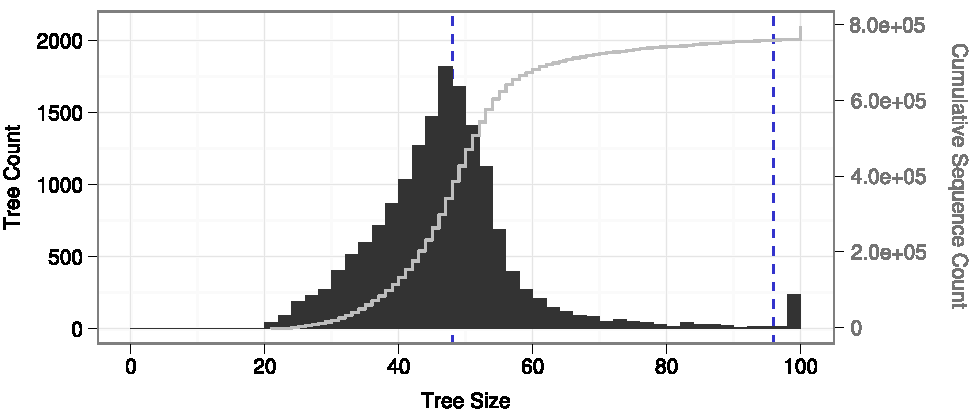
\includegraphics[scale=0.9]{Figs/hist_euth_roots.pdf}
\caption{Tree sizes for the set of \subtr{}s identified using the
  Eutheria clade taxonomic coverage constraint. Black bars show a
  histogram of tree sizes in bins of width 2, a gray line shows
  the cumulative number of sequences contained within trees of that
  size or smaller, and dashed blue lines are drawn at integral
  multiples of 48, the number of vertebrate species within
  Ensembl. Trees with more than 100 sequences are included in the
  topmost bin.}
\label{fig_ensembl_euth_hist}
\end{figure}

The distribution of tree sizes for the set of Eutherian \subtr{}s is
shown in Figure \ref{fig_ensembl_euth_hist}. The histogram of tree sizes
showed a single peak at exactly the number of vertebrate species in
\ens, with no trees containing fewer than 20 sequences and a few
hundred trees with more than 100 sequences. The distribution of tree
sizes was consistent with the set of 16,477 gene trees representing an
accurate set of genome-wide \mammln \acp{lot}, with variations in
sequence counts resulting from sporadic gene duplication or loss
events or unannotated genes in \lcv genomes.

\bbfig
\centering
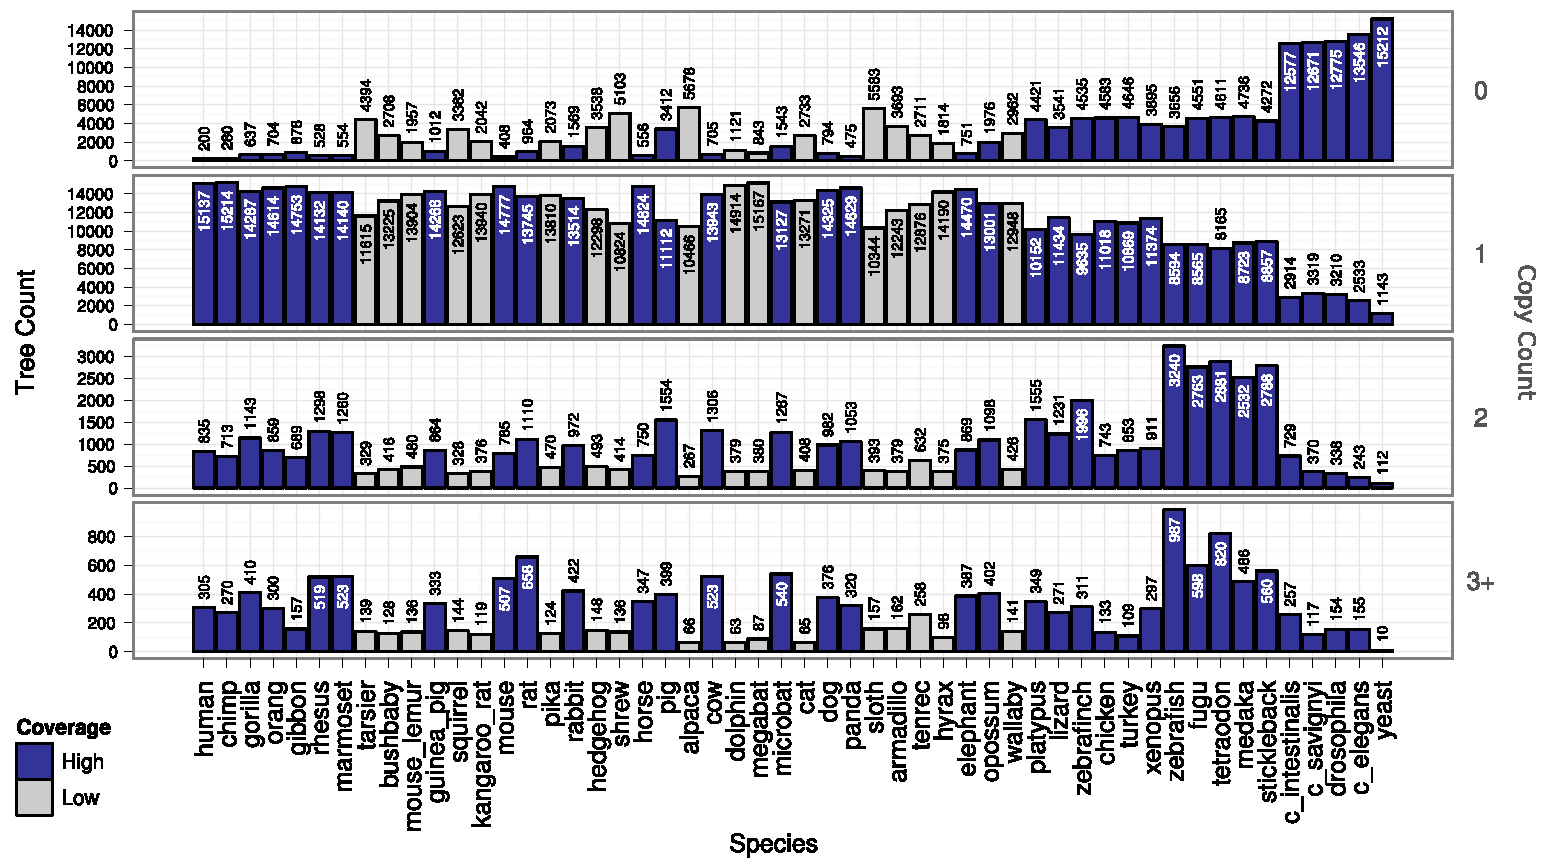
\includegraphics[scale=0.83]{Figs/dups_euth_roots.pdf}
\caption{Taxonomic distribution of gene copy counts for the Eutheria
  \subtr{}s defined by taxonomic coverage constraints. Results for the
  Primates, Glires, and Laurasiatheria are omitted for clarity; they
  showed similar characteristics to the Eutheria, Amniotes, and
  Vertebrata methods \ref{ensembl_subtree_table}). Each panel from top
  to bottom shows the number of trees containing 0, 1, 2 or more than
  3 sequences from each species. Bars are colored blue and gray for
  species with high- and low-coverage genomes, respectively. Note that
  the y-axis scale is not the same for each panel.}
\label{fig_ortholog_euth_dups}
\eefig

I also analyzed the detailed taxonomic distribution of gene
duplications and losses implied by the set of Eutherian \subtr{}s, as
the relative prevalence of zero-copy and multi-copy trees in this set
of \acp{lot} might provide some indication of whether gene deletion or
gene duplication has been more prevalent in the evolution of
vertebrate genomes. Figure \ref{fig_ortholog_euth_dups} shows the gene
copy counts for the set of Eutherian \subtr{}s across all \ens
species, similar to what Figure \ref{ortholog_root_dups} showed for
the set of root \cmp gene trees. The excess of \zcop trees and deficit
of duplications in \lcv genomes is immediately apparent from Figure
\ref{fig_ortholog_euth_dups}, confirming the trend observed in the set
of root \cmp trees. Similarly, the trend of increased \zcop trees in
non-mammalian and non-vertebrate species was stronger than in Figure
\ref{ortholog_root_dups}, as was the excess of trees with multiple
copies in fish genomes.

A quantitative comparison of the number of multi-copy versus zero-copy
trees in each species showed that gene duplication has had a greater
apparent impact on gene copy counts than gene deletion, at least
within primates and most mammals with high-coverage genomes. For
example, human contained 200 zero-copy trees and 1,140 combined two-
or three-copy trees within the set of Eutherian \subtr{}s, showing
evidence for a greater prevalence of gene duplication than gene
deletion in \acp{lot} since the common Eutherian ancestor. On the
other end of the spectrum in primates was gibbon, which had the most
\zcop trees (878) and the fewest multi-copy trees (846) of all the
primates, showing roughly equal tendencies towards gene deletion and
duplication across the set of Eutherian \acp{lot}. This pattern was
consistent across the mammalian tree, save for a few exceptions:
guinea pig showed roughly the same number of zero-copy and multi-copy
trees (1012 vs.~1197, respectively), rabbit showed slightly more
zero-copy trees (1569 vs.~1394), and pig showed a much higher number
of zero-copy trees (3412 vs. 1953). Beginning with opossum,
vertebrates more distantly related to the Eutherian common ancestor
showed greater numbers of \zcop trees, leveling off at ca.~4,000
zero-copy trees, and higher variation in the number of multi-copy
trees; at the low end were chicken and turkey with 876 and 972
multi-copy trees, respectively, and at the high end (excluding the
fish species) were zebrafinch and platypus with 1904 and 2307
multi-copy trees, respectively.

In the analysis of vertebrate genomes, one must be aware of potential
biases arising from the frequent reliance on homology with the
well-annotated human and mouse genomes in the annotation of newly
sequenced genomes. Such a bias could have plausibly led to anomalous
results in the present analysis of gene copy counts, for example by
reducing the chance of correctly identifying gene trees containing
deletions in human or mouse, thus over-inflating the prevalence of
duplications versus deletions. The level of consistency seen in the
relative numbers of \zcop and multi-copy trees across the range of
mammals provided some evidence against such a bias, although it did
not entirely rule out the possibility, as all mammalian genomes may
have been similarly affected by the use of human or mouse proteins in
the \ens gene annotation pipeline.

An unexpected result of the comparison between mammalian species was
the identification of certain genomes with uncharacteristically high
numbers of \zcop or multi-copy trees. The most striking example was
pig, which contained nearly double the number of \zcop trees of any
other high-coverage \mammln genome and a noticeably elevated number of
multi-copy trees, but rabbit and guinea pig also deviated from the
normal patterns. Given the otherwise consistently low number of \zcop
trees throughout the range of Eutherian mammals, I would expect the
number of \zcop trees in these species to decrease as finished-quality
genome sequences are produced and the gene annotation pipelines are
further optimized to work with each species. In particular the
anomalous nature of the pig gene trees may be related to the draft
quality of the genome sequence and assembly; I would expect the number
of \zcop trees to be substantially reduced once a finished-quality
genome sequence and annotation set is made available
\citep{Archibald2010}.


\section{Comparison to gene trees from the OPTIC database of amniote orthologs}

\begin{figure}
\centering
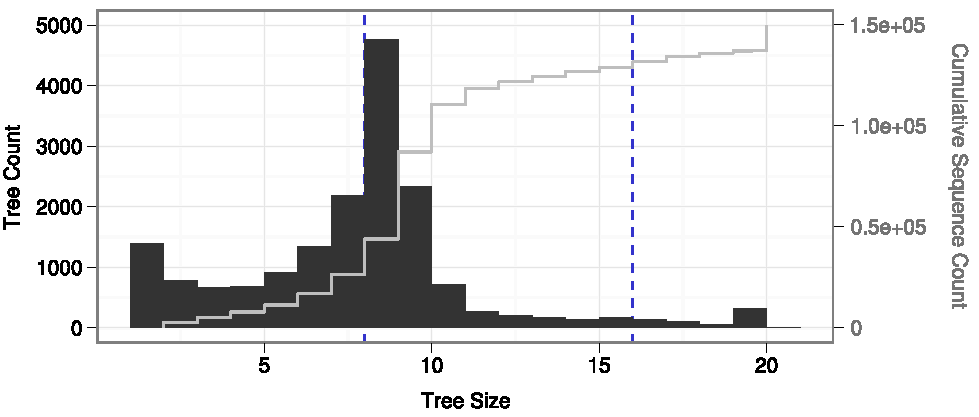
\includegraphics[scale=0.9]{Figs/hist_optic_roots.pdf}
\caption{Tree sizes for gene trees in eight amniote species from
  the OPTIC orthology database \citep{Heger2008}. Black bars show a
  histogram of tree sizes, a gray line shows the cumulative
  number of sequences contained within trees of that size or
  smaller, and dashed blue lines are drawn at integral multiples of 8,
  the number of amniote species analyzed by OPTIC. Trees with more
  than 20 sequences are included in the topmost bin.}
\label{fig_optic_roots_hist}
\end{figure}

Given the tendency of the root \cmp gene trees to contain multiple
\mammln \acp{lot}, I wished to evaluate whether a different
phylogenetic tree-based orthology pipeline produced a similar
distribution of gene tree sizes. The OPTIC database, a project from
Christ Ponting's group which used an independently designed
gene-building and comparative genomics pipeline combined with the
TreeBeST software to infer duplication-resolved gene trees within a
variety of vertebrate and invertebrate clades, was ideal for such a
comparison \citep{Heger2008}. I downloaded the set of OPTIC gene trees
inferred from a group of eight vertebrate genomes (human, mouse, dog,
opossum, platypus, chicken, zebrafinch, and tetraodon), characterized
the set of gene trees using a variety of summary statistics (included
in the bottom row of Table \ref{ensembl_subtree_table}) and plotted the
distribution of gene tree sizes in Figure \ref{fig_optic_roots_hist}.

After accounting for differences in the number of sampled species, the
set of OPTIC gene trees more closely resembled the set of Eutherian
\subtr{}s than the root \cmp gene trees (Table
\ref{ensembl_subtree_table}). Nearly 80\% of the OPTIC gene trees
contained exactly one human sequence and only 9\% contained two or
more human sequences; the large proportion of single-copy trees
suggested that the OPTIC trees did not contain many ``over-clustered''
\mammln \acp{lot}, and the 9\% of trees with multiple human genes was
close to the 7\% seen in the set of Eutherian \subtr{}s. Figures
\ref{fig_ensembl_euth_hist} and \ref{fig_optic_roots_hist} clearly show that
the OPTIC and Eutherian trees contain similarly-shaped distributions
of sequence counts; each histogram has a distinct peak at a sequence
count corresponding to the number of species included in the database,
with no sign of the long tail of large gene trees seen for the
distribution of root \cmp gene trees in Figure
\ref{fig_ensembl_roots_hist}.

\section{Conclusions}

This chapter was concerned with identifying a set of \acfp{lot} for use
in a downstream analysis of \sw selective pressures in mammalian
orthologs. Three characteristics were desired in the ideal set of
trees: maximal coverage of available mammalian genomes, minimal
inclusion of paralogous relationships, and consistent taxonomic
representation throughout the set of trees. The \ens \cmp database as
a source of inferred gene trees due to its well-established
methodology \citep{Heger2008,Vilella2009} and because genes from \lcv
mammalian genomes were included in the inference pipeline, resultin
gin increased species sampling compared to equivalent vertebrate
databases such as Treefam and OPTIC.

Using the set of root \cmp gene trees as a basis for further analysis,
I characterized the distribution of gene trees in a variety of ways,
including using a tree-based analogue of the N50 statistic commonly
used in evaluating genome assemblies. This analysis showed that the
``over-clustering'' of multiple Eutherian \acp{lot} within single \cmp
gene trees had a major impact on the composition of the gene tree
set. I then developed a simple scheme for isolating \acp{lot} from
within larger gene trees using flexible \acfp{tcc} and applied the
method to the set of \cmp trees to generate several sets of
genome-wide \ac{tc}-defined \subtr{}s.

These sets of \ac{tc}-defined \subtr{}s provided a number of insights
into the orthology and paralogy relationships within and between
mammalian and vertebrate genomes, including a quantification of the
proportion of duplicate genes that were retained after the teleost
whole-genome duplication that matched the prediction resulting from a
detailed analysis of fish genomes \citep{Brunet2006}. The comparison
between \subtr{} sets resulting from different \acp{tcc} showed that a
simple threshold based on \ac{tc} in the Eutheria clade produced a set
of \subtr{}s that contained a high percentage of human genes and
satisfied the three desired characteristics for subsequent sitewise
analysis.

Analysis of the number of trees with zero, one, two or more sequences
for a given species revealed patterns of variation in gene copy counts
across vertebrate genomes. Importantly, \lcv genomes showed a large
increase in zero-copy trees (e.g. trees with no sequences from the
low-coverage genome) and a notable decrease in multi-copy trees. The
increased number of zero-copy trees reflected an expected amount of
loss resulting from missing sequence data in \lcv genomes and was not
too worrying with respect to the intended downstream analysis. The
decreased number of multi-copy genes was concerning, however, as it
suggested that the assembly of duplicated genomic regions may
frequently be ``collapsed'' in \lcv assemblies, possibly resulting in
genes containing chimeric sequence derived from different duplicated
segments.

Other, more subtle trends in the patterns of gene copy counts were
identified, including individual genomes, such as pig, with apparently
anomalous numbers of zero- or multi-copy trees, and more widespread
trends, such as the relatively few multi-copy trees in avian genomes
and the higher prevalence of multi-copy trees versus zero-copy trees
within mammals.

A major conclusion of the analysis presented in this chapter was that
the use of taxonomic criteria is important in identifying mammalian
\acp{lot}. Other gene tree databases, such as TreeFam
\citep{Ruan2008} and OPIC \citep{Heger2008} explicitly use taxonomic
information or outgroups to ensure that orthologs are consistently
clustered, but \cmp currently does not use such information in
building its gene trees. As a result, I developed a simple method to
extract \ac{lot} from the set of ``root'' \cmp trees and evaluated the
method by analyzing the distribution of tree sizes, the number of
human gene copies per tree, and the taxonomic distribution of gene
copy counts for the \ac{tc}-defined \ac{lot} compared to the ``root''
\cmp trees. Further comparison of these statistics to a separate
dataset of amniote orthologs provided confirmation that the resulting
trees more closely resembled previously-published sets of orthologous
groups.

One might argue that a gene tree with fully-resolved duplication and
speciation events, as provided by the \cmp database, should be enough
to allow for identification of orthologous versus paralogous
\subtr{}s. In theory this is true, but such an approach to identifying
\acp{lot} would have failed on two grounds: first, it would not
distinguish between ancient paralogs resulting from the two rounds of
whole-genome duplication in vertebrates and more recent paralogs
resulting from the gradual accrual of gene duplications over time,
causing recent duplication events to be handled in the same way as
ancient duplications absent the incorporation of taxonomic
information. Second, in practice the resolution of gene deletions
within the \cmp gene trees was far from perfect, a point raised by
Milinkovitch et al. \citeyearpar{Milinkovitch2010} in their criticism
of the inclusion of \lcv genomes in the \ens \cmp orthology
pipeline. A lack of data, caused either by missing genes from \lcv
genomes or by the limited amount of sequence data available for
phylogenetic reconstruction, may often contribute to errors in the
accurate identification of duplication and speciation nodes within the
\cmp gene trees; in a sense, the use of \ac{tc} information avoided
this source of uncertainty by not relying on accurate resolution of
individual duplication events.
